\section{Supporting qualification evidence}
\label{app:res-evidence}
This appendix preserves the detail needed to interpret the main qualification tests without repeating the Design's subsystem derivations. The separate supporting-evidence package contains the original v6 measurement archive, reviewed records and figure-generation scripts. Newly computed analyses are identified separately from the original measurements. No physical measurement is generated by a plotting script.

\subsection{Evaluated checkpoints and populations}
The selected demonstration reader is the library-trained joint reader, as confirmed by the author. The numerical scratch reader is a comparison model. The selected writer model is the library-trained eleven-writer 0.17 model. Table~\ref{tab:app-checkpoints} records hash prefixes; the evidence manifest retains the full SHA-256 values. A filename alone is insufficient because the archived reader study identified two different files named \texttt{scratch\_best}.

\begin{table}[!htbp]\centering\small
\begin{tabular}{lll}\toprule
\textbf{Role} & \textbf{Checkpoint identifier} & \textbf{SHA-256 prefix}\\\midrule
Selected reader & joint\_best & \texttt{336802d535992323}\\
Comparison reader & evaluated scratch\_best & \texttt{2add315ded078de5}\\
Selected writer & 11\_pw170 & \texttt{1884fb86467538eb}\\
Comparison writer & 11w\_pw170\_scratch & \texttt{b23a709a30144f67}\\\bottomrule
\end{tabular}
\caption{Identities of the measured model files.}\label{tab:app-checkpoints}\end{table}

The numerical-writer training excerpt supplied by the author records 1\,031 training lines and 155 validation lines, 0.17 normalisation, a 50-epoch budget and a best displayed validation accuracy of 0.968 by epoch 41. The retained excerpt continues through epoch 47 and does not document a completed epoch 50. Its later common-set score is measured on 156 re-extracted validation lines; the different population is retained rather than silently equated with training validation. The numerical-reader excerpt records 6\,481 public training lines, 569 personal training lines, 976 public validation lines and 100 personal validation lines, and a resume from an existing checkpoint. These are training-history records, while QT~2 evaluates saved weights directly.

An additional inventory reads each selected stored profile and verifies nonempty glyph mappings. The numbers of distinct character keys are 42, 38, 37, 36, 40 and 41 for the six database writers, and 56, 42, 43, 42 and 58 for A, B, O, T and Y. All eleven names agree with the selected writer checkpoint. The full source paths and content hashes are preserved in \texttt{ResultsEvidence/profile\_inventory.json}. These counts establish stored mappings; they do not imply equal coverage of every character in the reader alphabet.

\subsection{Reader validation breakdown}
Table~\ref{tab:app-reader-breakdown} extends the population totals in QT~2. The personal contributors are retained separately, using the same reader checkpoints and greedy decoder.
\begin{table}[!htbp]\centering\small
\begin{tabular}{lrrrr}\toprule
\textbf{Evaluation set} & \textbf{Lines} & \textbf{Characters} & \textbf{Joint / \%} & \textbf{NumPy / \%}\\\midrule
Public IAM validation & 976 & 42072 & 94.12 & 94.39\\
Photographed A & 31 & 934 & 94.00 & 94.65\\
Photographed B & 19 & 739 & 95.81 & 97.70\\
Photographed O & 22 & 1017 & 94.40 & 94.79\\
Photographed T & 11 & 345 & 85.51 & 89.28\\
Photographed Y & 17 & 640 & 92.03 & 92.50\\
All & 1076 & 45747 & 94.06 & 94.39\\
\bottomrule\end{tabular}
\caption{Reader character accuracy by validation population.}\label{tab:app-reader-breakdown}
\end{table}

\subsection{Physical reproduction by writer}
\begin{table}[!htbp]\centering\small
\begin{tabular}{lrrrr}\toprule
\textbf{Writer} & \textbf{Lines} & \textbf{Character / \%} & \textbf{Writer / \%} & \textbf{Word match / \%}\\\midrule
Y & 13 & 97.01 & 92.31 & 74.16\\
150 & 13 & 96.75 & 53.85 & 76.40\\
O & 16 & 94.25 & 100.00 & 58.51\\
B & 16 & 93.11 & 93.75 & 68.24\\
384 & 16 & 86.93 & 87.50 & 43.18\\
552 & 15 & 86.17 & 80.00 & 48.39\\
152 & 15 & 85.74 & 80.00 & 49.44\\
A & 27 & 77.29 & 100.00 & 18.09\\
153 & 19 & 75.72 & 57.89 & 31.46\\
588 & 18 & 73.19 & 94.44 & 22.99\\
T & 16 & 60.97 & 100.00 & 13.41\\
\bottomrule\end{tabular}
\caption{Physical reproduction scores by writer.}\label{tab:app-r1-writers}
\end{table}

The paired read-back study contains 184 transcript-bearing lines. A separate model comparison contains 185 writer-labelled crops, including one crop with no corresponding transcript line. It can support a writer-prediction comparison, but that extra crop is not inserted into a character score. The model-comparison pooled groups are writers, not a claim that only eleven physical sheets were drawn.


\subsubsection{Per-line classification rates and the board-to-host projection}
The two ODROID classification requests are the only embedded records that
separate the reader from the writer namer. Restating their logged stage
seconds per line rather than per character uses the same two measurements and
no new one: $19.024/16$ and $24.658/22$ for the reader, $11.091/16$ and
$14.014/22$ for the namer. The per-line agreement, 5.9\% and 8.4\%, is much
closer than the per-character agreement of 41.0\% and 43.4\%, because both
networks are given one fixed $64\times640$ canvas for every line.

Host rates were then measured on ten photographed pages and 221 lines with
the deployed code and checkpoints, timing \texttt{SegmentLines} through its
own stage timer and then reading and naming every line crop, which is the
order and the work a request performs. Dividing the board rates by the host
medians gives the stage ratios quoted in Section~\ref{qt:r4}. The record,
including every per-page host figure and the leave-one-out check, is
\texttt{ResultsEvidence/measurements/} \texttt{host\_classify\_stage\_times\_2026-11-02.json}.

Three limits apply. The board was not available when this was prepared, so
nothing here is a new embedded measurement and every projected figure is
labelled as such. The ratio rests on two board observations. The
\texttt{reading back} stage recorded in the reproduction records is a
different measurement, one rendered or drawn line rather than a photographed
page, and is not pooled with these rates.

\subsection{New geometric style comparison on physical pages}
\label{app:res-physical-style}
The new analysis applies the archived descriptor definitions with the current segmentation primitives to 156 original reference lines and 184 physical-output lines. The original population consists of the same six held-out database pages and 100 seeded photographed reference lines used for writer evaluation. The physical population comprises all fourteen robot pages after the recorded orientation convention. Each page's crop count agrees with its transcript-bearing records, and every line returns usable descriptors. All eleven writers are retained.

Each line is binarised, its body band estimated and its image resized toward a 28-pixel body height before the descriptors are evaluated. The same procedure is applied to both domains. Writer means give equal weight to available lines for each feature, and the pooled correlation gives equal weight to writers and selected features. Word-gap values are absent where no qualifying gap exists: 155/156 original and 180/184 physical lines have a value; the other descriptors are available for every line. All eleven writer means remain usable. The within-domain variant separately standardises each feature in each domain; the absolute variant uses original-domain means and standard deviations for both. Source images, the personal-crop cache, scripts and full measurements are recorded by hash. The raw outputs are in \texttt{ResultsEvidence/physical\_style/results.json}.

The per-feature correlations are slant 0.9911; stroke width 0.7986; ink density 0.7392; word gap 0.4861; components per word 0.6688; character width 0.7978; ascender extent 0.8173; descender extent 0.5394; and extent ratio 0.5762. Figure~\ref{fig:app-physical-style} shows the actual writer means. Each point represents one writer, and dashed lines mark equal feature values. The 10\,000-repeat writer-resampling range for the seven-feature within-domain coefficient is 0.5555--0.8272, using seed 23539195. It is a sensitivity range over this writer set. This retrospective comparison does not use identical sentences between domains and should not be interpreted as a controlled perceptual-equivalence experiment.
\begin{figure}[!htbp]\centering
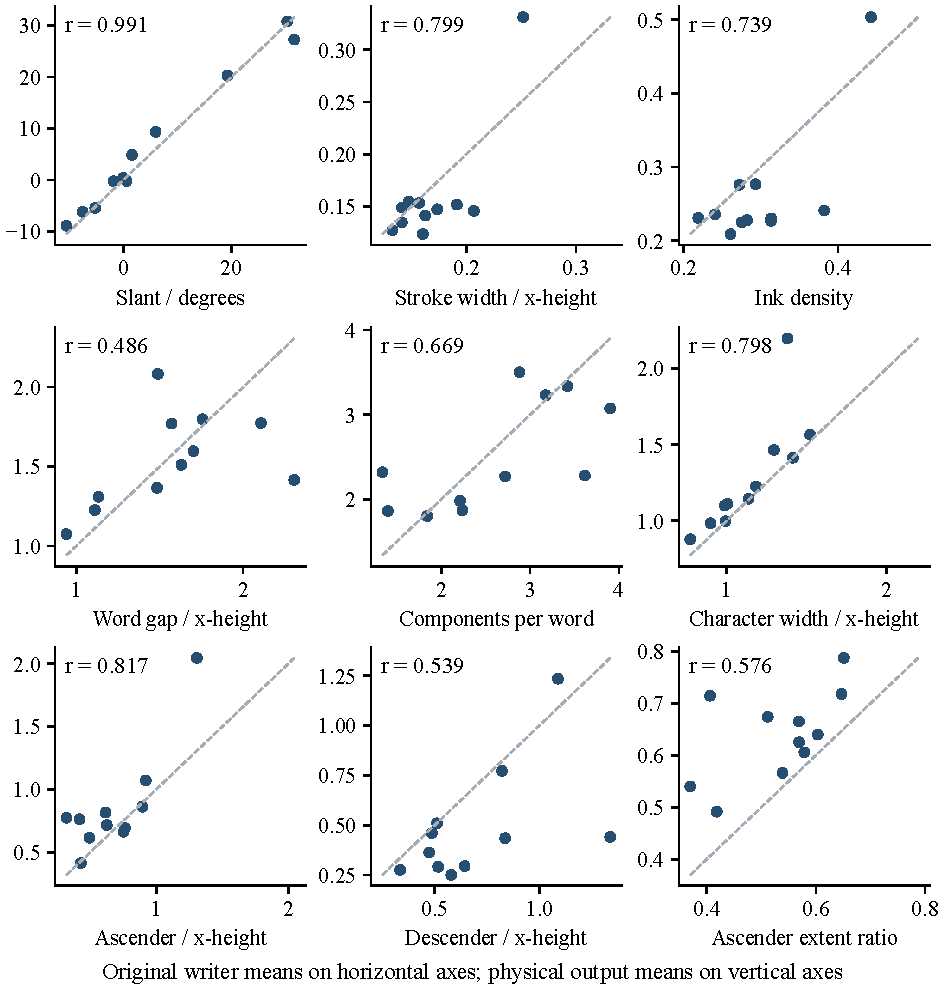
\includegraphics[width=\linewidth]{Figures/results_physical_style_scatter.pdf}
\caption{Original and reproduced writer descriptor means.}\label{fig:app-physical-style}\end{figure}

\subsection{Archived geometric style study}
\label{app:res-style}
The archived study covers writers 150, 151, 152, 153, 384, 551, 552, 588, B and Y. There are six synthetic lines per writer, sixty in total, compared with 123 original reference lines marked as excluded from profile building. This earlier ten-writer set differs from the final eleven-writer evaluation. The study is retained to explain geometric behaviour of the method; it is not relabelled as a measurement of final physical pages.

Nine deterministic descriptors measure slant, normalised stroke width, ink density, word gap, components per word, character width, ascender extent, descender extent and the ascender-to-total-extent ratio. Seven shape descriptors omit stroke width and ink density. The within-domain pooled correlation first standardises each feature across writers separately in the real and synthetic domains, then correlates the flattened arrays. It is therefore insensitive to a uniform offset or scale difference between those domains. The alternative absolute variant standardises both arrays using the real-domain mean and standard deviation. This distinction matters when interpreting preservation of magnitude rather than writer ordering.

\begin{table}[!htbp]\centering\small
\begin{tabular}{lrr}\toprule
\textbf{Feature set} & \textbf{Separate-domain standardisation} & \textbf{Real-domain standardisation}\\\midrule
Nine features & 0.7013 & 0.5994\\
Seven shape features & 0.7142 & 0.6711\\\bottomrule
\end{tabular}
\caption{Archived synthetic-to-original pooled correlations against the profile-held-out reference. The 0.714 value is the seven-shape-feature variant.}\label{tab:app-style-variants}\end{table}

The per-feature coefficients are 0.9964 for slant, 0.6315 for stroke width, 0.6802 for ink density, 0.6050 for word gap, 0.8323 for components per word, 0.9358 for character width, 0.9735 for ascender extent, 0.1480 for descender extent and 0.5085 for the extent ratio. Correlation describes variation across writers; it does not prove pointwise agreement of all letter shapes. The recorded 2\,000 writer-resample interval for the seven-feature within-domain result is 0.6118--0.8586.

The archived overlay experiment uses thirty source texts across those ten writers. With x-height normalisation, mean matched chamfer distance is 0.6302, mean mismatched distance is 1.3868, their ratio is 2.2007 and the recorded AUC is 0.7074. When the archive also applies its width-normalisation variant, AUC is 0.4630. Thus the favourable separation depends on the chosen normalisation; an AUC above 0.5 in one variant must not be presented as universal writer fidelity. These remain software comparisons, without a new independent human panel.

\subsection{Timing selection and optimisation scope}
\label{app:res-speed}
QT~3 uses a deliberately checkable completion boundary. The earlier archive retained 36 records after deduplication and a drawing-rate filter. The revised primary count uses 25 positive-character console records with explicit program-end evidence. The original 36-record aggregation remains in the preserved provenance document. A rate threshold alone does not establish completion: a job stopped after substantial drawing can exceed that threshold. This change does not alter the observed worst 3.875~s per character. A terminal marker confirms the interpreter finished, while geometry and content remain separate qualification questions.

The 500- and 982-character counts for QT~4 are the counts printed in the timer record. A final repeat should retain independent transcript lengths and an acquisition-to-output timing boundary. The two current overruns are large, so no inferred sub-second camera transfer time is added to create a favourable pass.

\begin{table}[!htbp]\centering\small
\begin{tabularx}{\linewidth}{lX}\toprule
\textbf{Comparison} & \textbf{Measured outcome and scope}\\\midrule
Sequential NumPy vs batched library networks & 359.8~s vs 130.3~s over fourteen stored pages on the development host; factor 2.76. Both backend and batching change. Reader text is identical; writer-label equivalence is not inferred from that fact.\\[4pt]
Full vs half linear image resolution & 4.37-fold recorded image-stage factor on comparable successful page pairs, with 247 vs 182 detected lines. Zero of twelve comparable pages retain line count; two of fourteen reduced pages fail segmentation.\\[4pt]
Projected network-only replacement & Applying 2.76 to ODROID network stages, with image stages unchanged, gives approximately 27.05~s and 30.82~s. Neither is an observed ODROID result or a total-time pass.\\[4pt]
Projected combined replacement & Applying both host factors gives approximately 14.61~s and 17.86~s. The second is numerically below its allowance, but the image reduction changes the output and the timing is transferred between hosts. It is not accepted as R4 compliance.\\\bottomrule
\end{tabularx}
\caption{Acceleration evidence and the boundary between a measured comparison and a projected compliant configuration.}\label{tab:app-acceleration}\end{table}

The G-code study of the same 378-character paragraph yields pen-down path lengths from 2\,015.4 to 3\,942.8~mm and recorded pen-state counts from 544 to 1\,188 across eleven profiles. These are arithmetic properties of generated paths. They demonstrate profile-dependent geometry and help explain timing variation; they are not independent proof of similarity to genuine handwriting, and their values can still be affected by the candidate-selection process.

\subsection{Cost, consent and final records}
The photographed ledger supplied by the author is retained as evidence. The present build estimate is approximately R4\,000, with a borrowed ODROID entered at zero purchase cost. The later listed clipboard (R90), paper (R130), gel pen (R30) and estimated training electricity (R500) total R750. Their overlap with the approximate build estimate is not established, so they are not added to produce an unsupported exact total. Replacement value and estimated operating costs should be distinguished from actual purchased parts.

Signed consent forms are held by the author for the five personal contributors. The report records that fact without reproducing signatures. Participant consent is recorded separately from institutional clearance or exemption.

\subsection{Supporting timing and dimensional figures}
Figure~\ref{fig:res-r3} compares the worst completed reproduction total at each tested length with its allowance. Labels retain the number of records.
\begin{figure}[!htbp]\centering
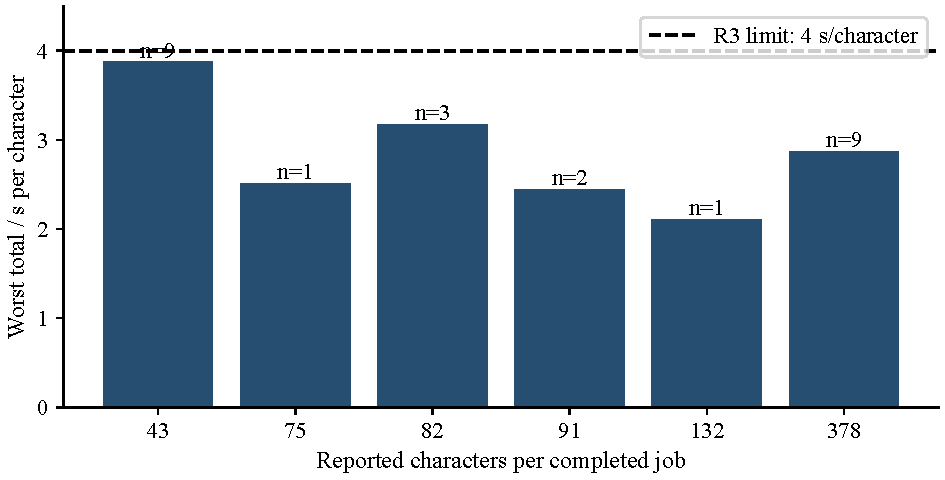
\includegraphics[width=\linewidth]{Figures/results_r3_confirmed.pdf}
\caption{Completed reproduction times and allowances.}
\label{fig:res-r3}\end{figure}
Figure~\ref{fig:res-r4} separates image and network processing for the two ODROID requests. The dashed markers show their complete allowances.
\begin{figure}[!htbp]\centering
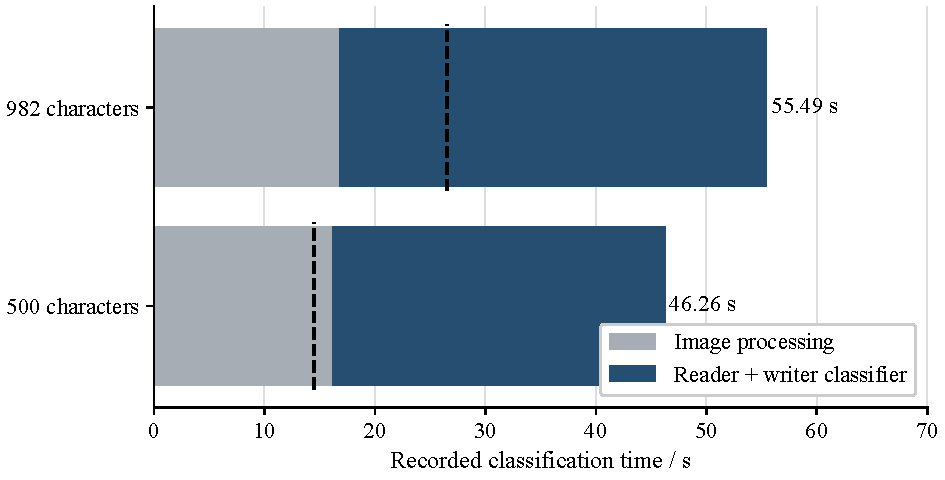
\includegraphics[width=\linewidth]{Figures/results_r4_stages.pdf}
\caption{ODROID classification stages and allowances.}
\label{fig:res-r4}\end{figure}
Figure~\ref{fig:res-geometry} compares each measured feature length with its nominal value. The dashed limits apply to length differences and do not establish absolute bed coordinates.
\begin{figure}[!htbp]\centering
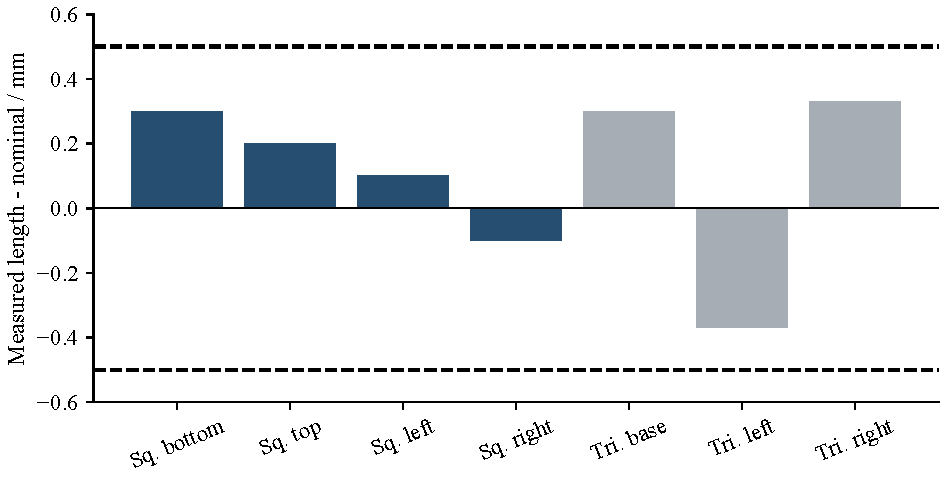
\includegraphics[width=\linewidth]{Figures/results_geometry_errors.pdf}
\caption{Signed errors in the measured feature lengths.}
\label{fig:res-geometry}\end{figure}

\subsection{Triangle geometry diagnostic}\label{app:res-geometry-calculation}
Place the measured base endpoints at $(-b/2,0)$ and $(b/2,0)$ and the apex at $(d,h)$. Subtracting the two squared-distance equations gives the project's geometric diagnostic:
\begin{equation}
d=\frac{\ell^2-r^2}{2b},\qquad \phi_{\rm app}=\arctan(d/h).
\label{eq:res-apex}
\end{equation}
Using $b=80.30$~mm, $\ell=56.20$~mm, $r=56.90$~mm and the nominal $h=40$~mm gives $d=-0.493$~mm and $\phi_{\rm app}=-0.706^\circ$. The angle is conditional on the assumed height and a shear interpretation; it is not an independent measurement of rail squareness. Both an ideal square and a rhombus can have equal side lengths, which is why diagonal or coordinate measurements would add information absent from the square-side test.


\subsection{Complete physical-page records}\label{app:res-page-records}
Table~\ref{tab:app-pages} retains all fourteen pages. Photographs are rotated for reading without changing their image data. Character accuracy pools edit counts within each page. Writer identification uses its paired lines. Text and timing records have no verified one-to-one job link, so the timing table below is kept separate.
\begin{longtable}{lrrrrr}
\caption{All physical pages and paired-line scores.}\label{tab:app-pages}\\
\toprule Page & Lines & Characters & Edits & Character / \% & Writer / \%\\\midrule\endfirsthead
\toprule Page & Lines & Characters & Edits & Character / \% & Writer / \%\\\midrule\endhead
Author150 & 13 & 493 & 16 & 96.75 & 53.85\\
Author152 & 15 & 491 & 70 & 85.74 & 80.00\\
Author1531 & 15 & 407 & 106 & 73.96 & 60.00\\
Author1532 & 4 & 79 & 12 & 84.81 & 50.00\\
Author3841 & 13 & 409 & 52 & 87.29 & 92.31\\
Author3842 & 3 & 73 & 11 & 84.93 & 66.67\\
Author552 & 15 & 506 & 70 & 86.17 & 80.00\\
Author588 & 18 & 496 & 133 & 73.19 & 94.44\\
AuthorA1 & 17 & 361 & 82 & 77.29 & 100.00\\
AuthorA2 & 10 & 163 & 37 & 77.30 & 100.00\\
AuthorD & 16 & 479 & 33 & 93.11 & 93.75\\
AuthorO & 16 & 539 & 31 & 94.25 & 100.00\\
AuthorT & 16 & 474 & 185 & 60.97 & 100.00\\
AuthorY & 13 & 501 & 15 & 97.01 & 92.31\\
\bottomrule\end{longtable}

Figure~\ref{fig:app-physical-pages-1} preserves the photographed pages Author150, Author152. The scores come from their paired line records, not a visual estimate.
\begin{figure}[!htbp]\centering
\begin{minipage}{.48\linewidth}\centering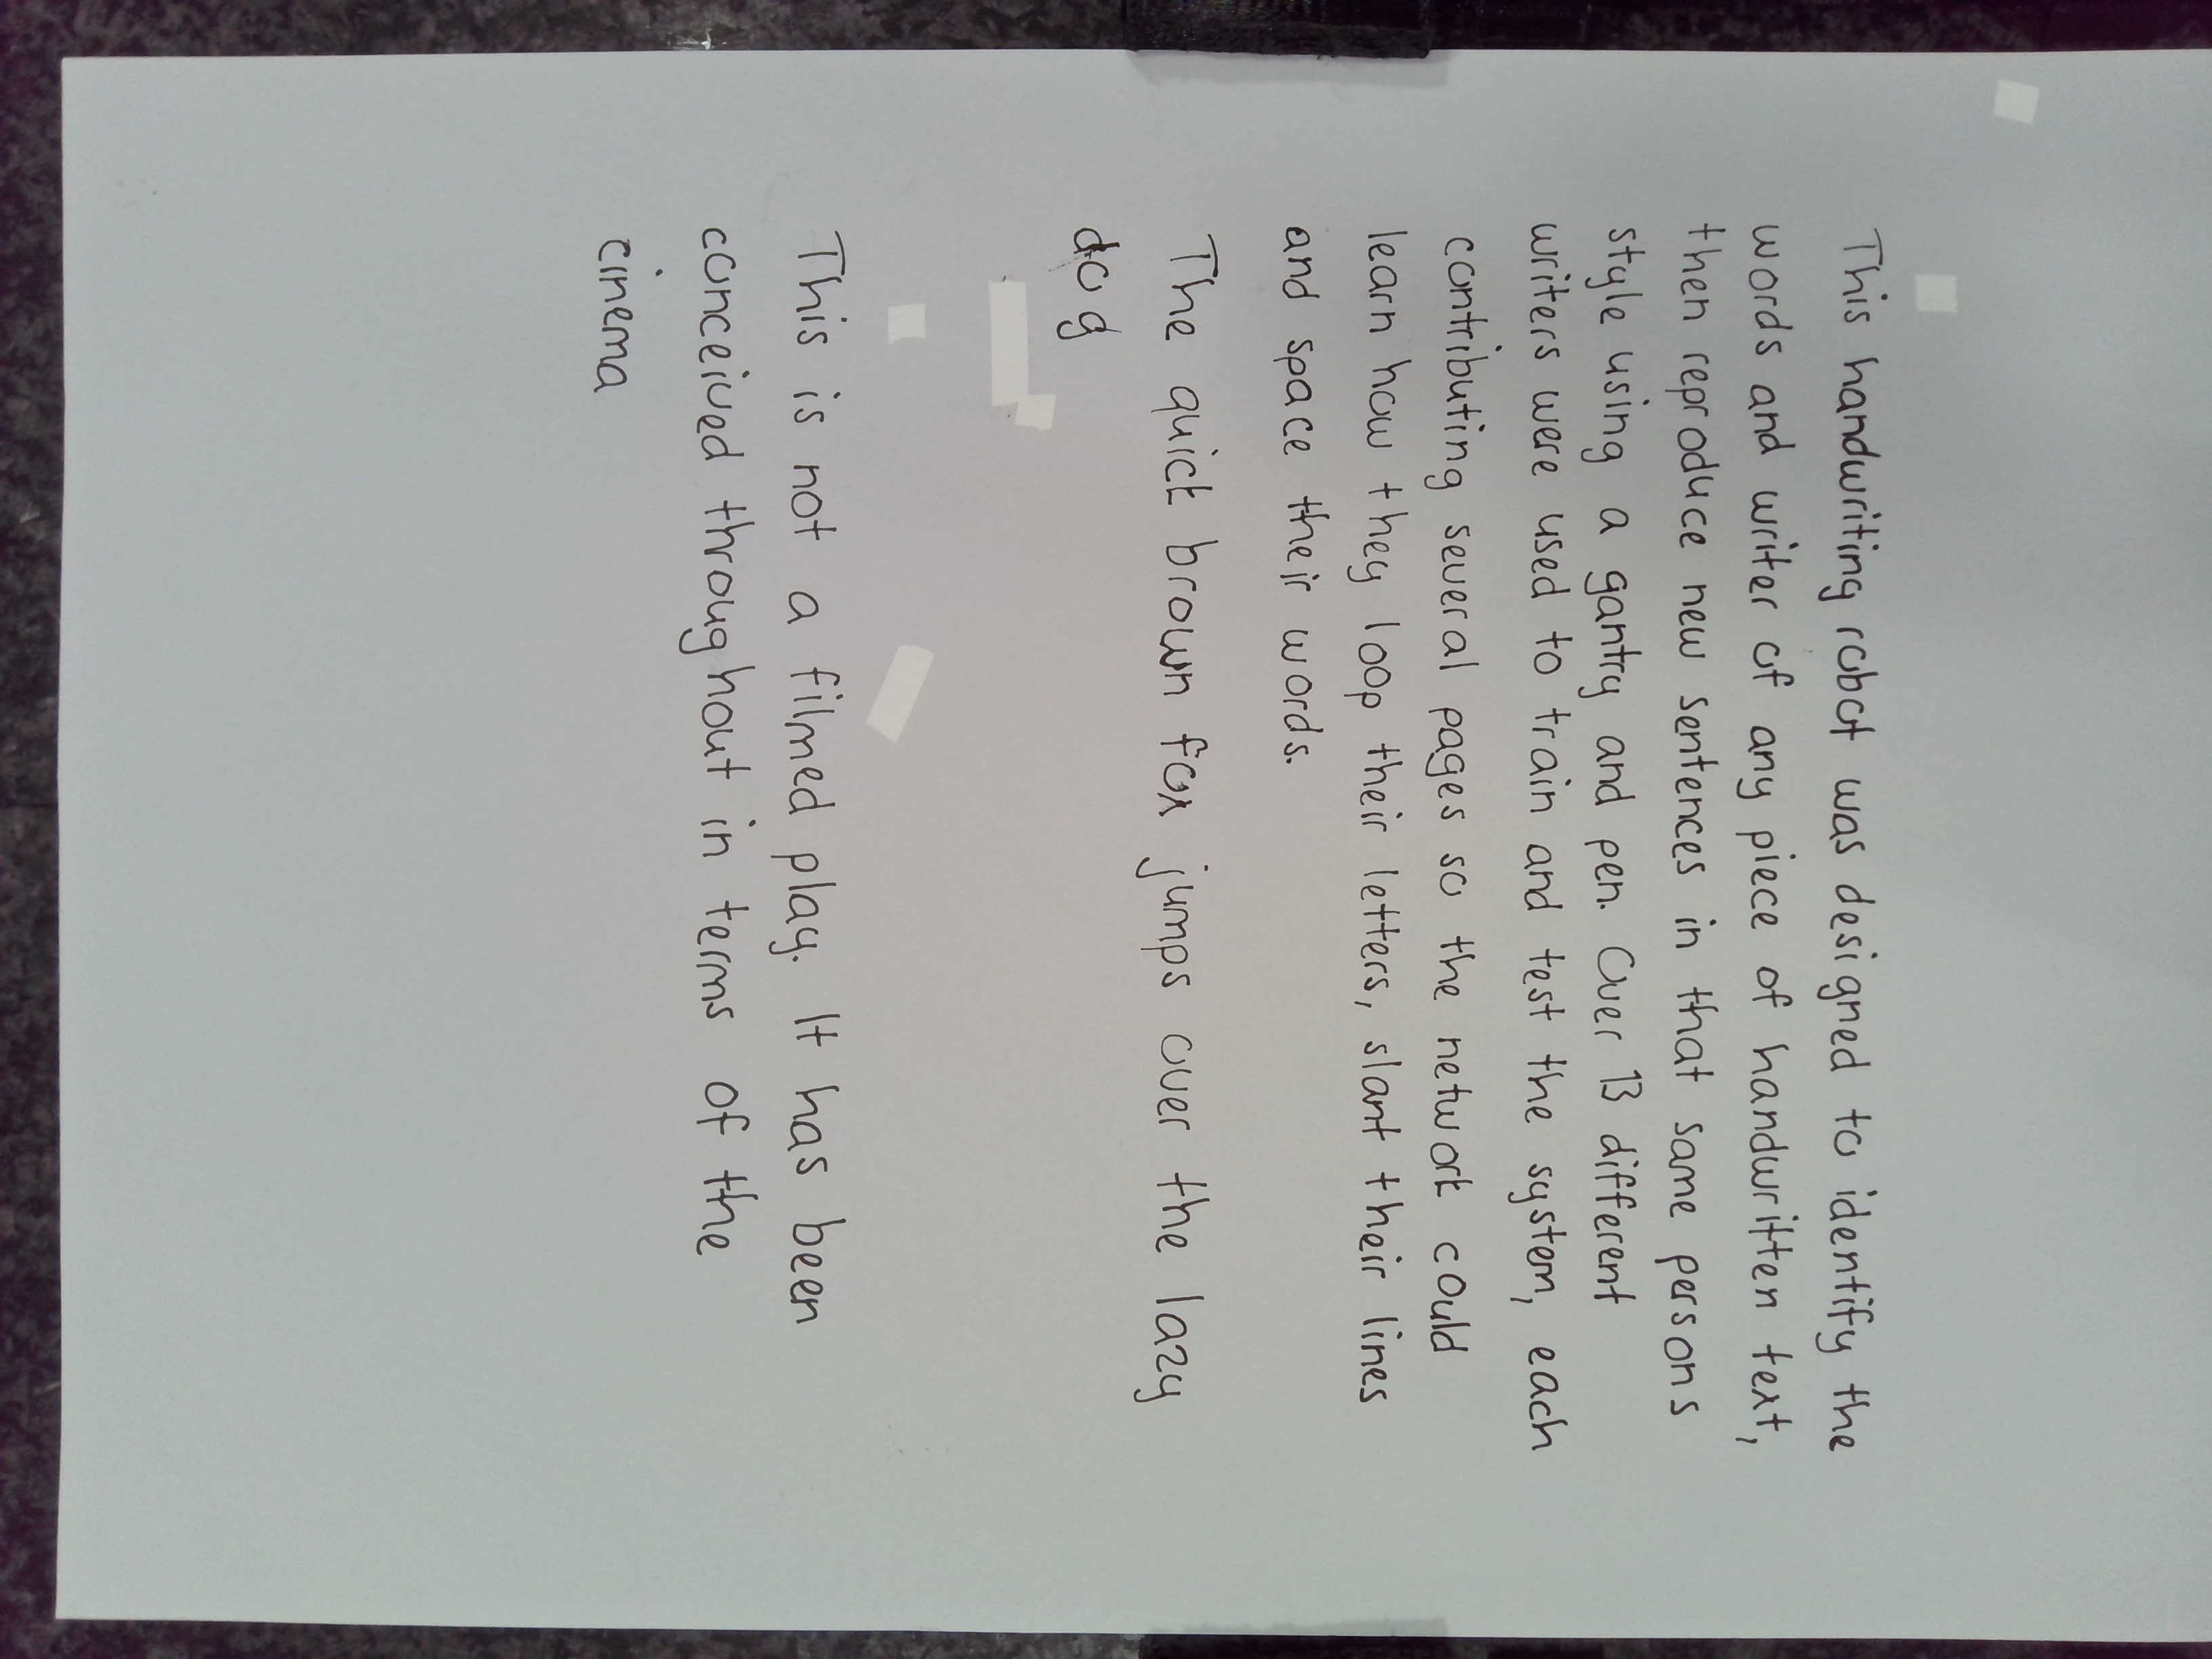
\includegraphics[angle=90,width=\linewidth,height=.55\textheight,keepaspectratio]{Figures/PhysicalPages/Author150.jpg}\par Author150\end{minipage}\hfill
\begin{minipage}{.48\linewidth}\centering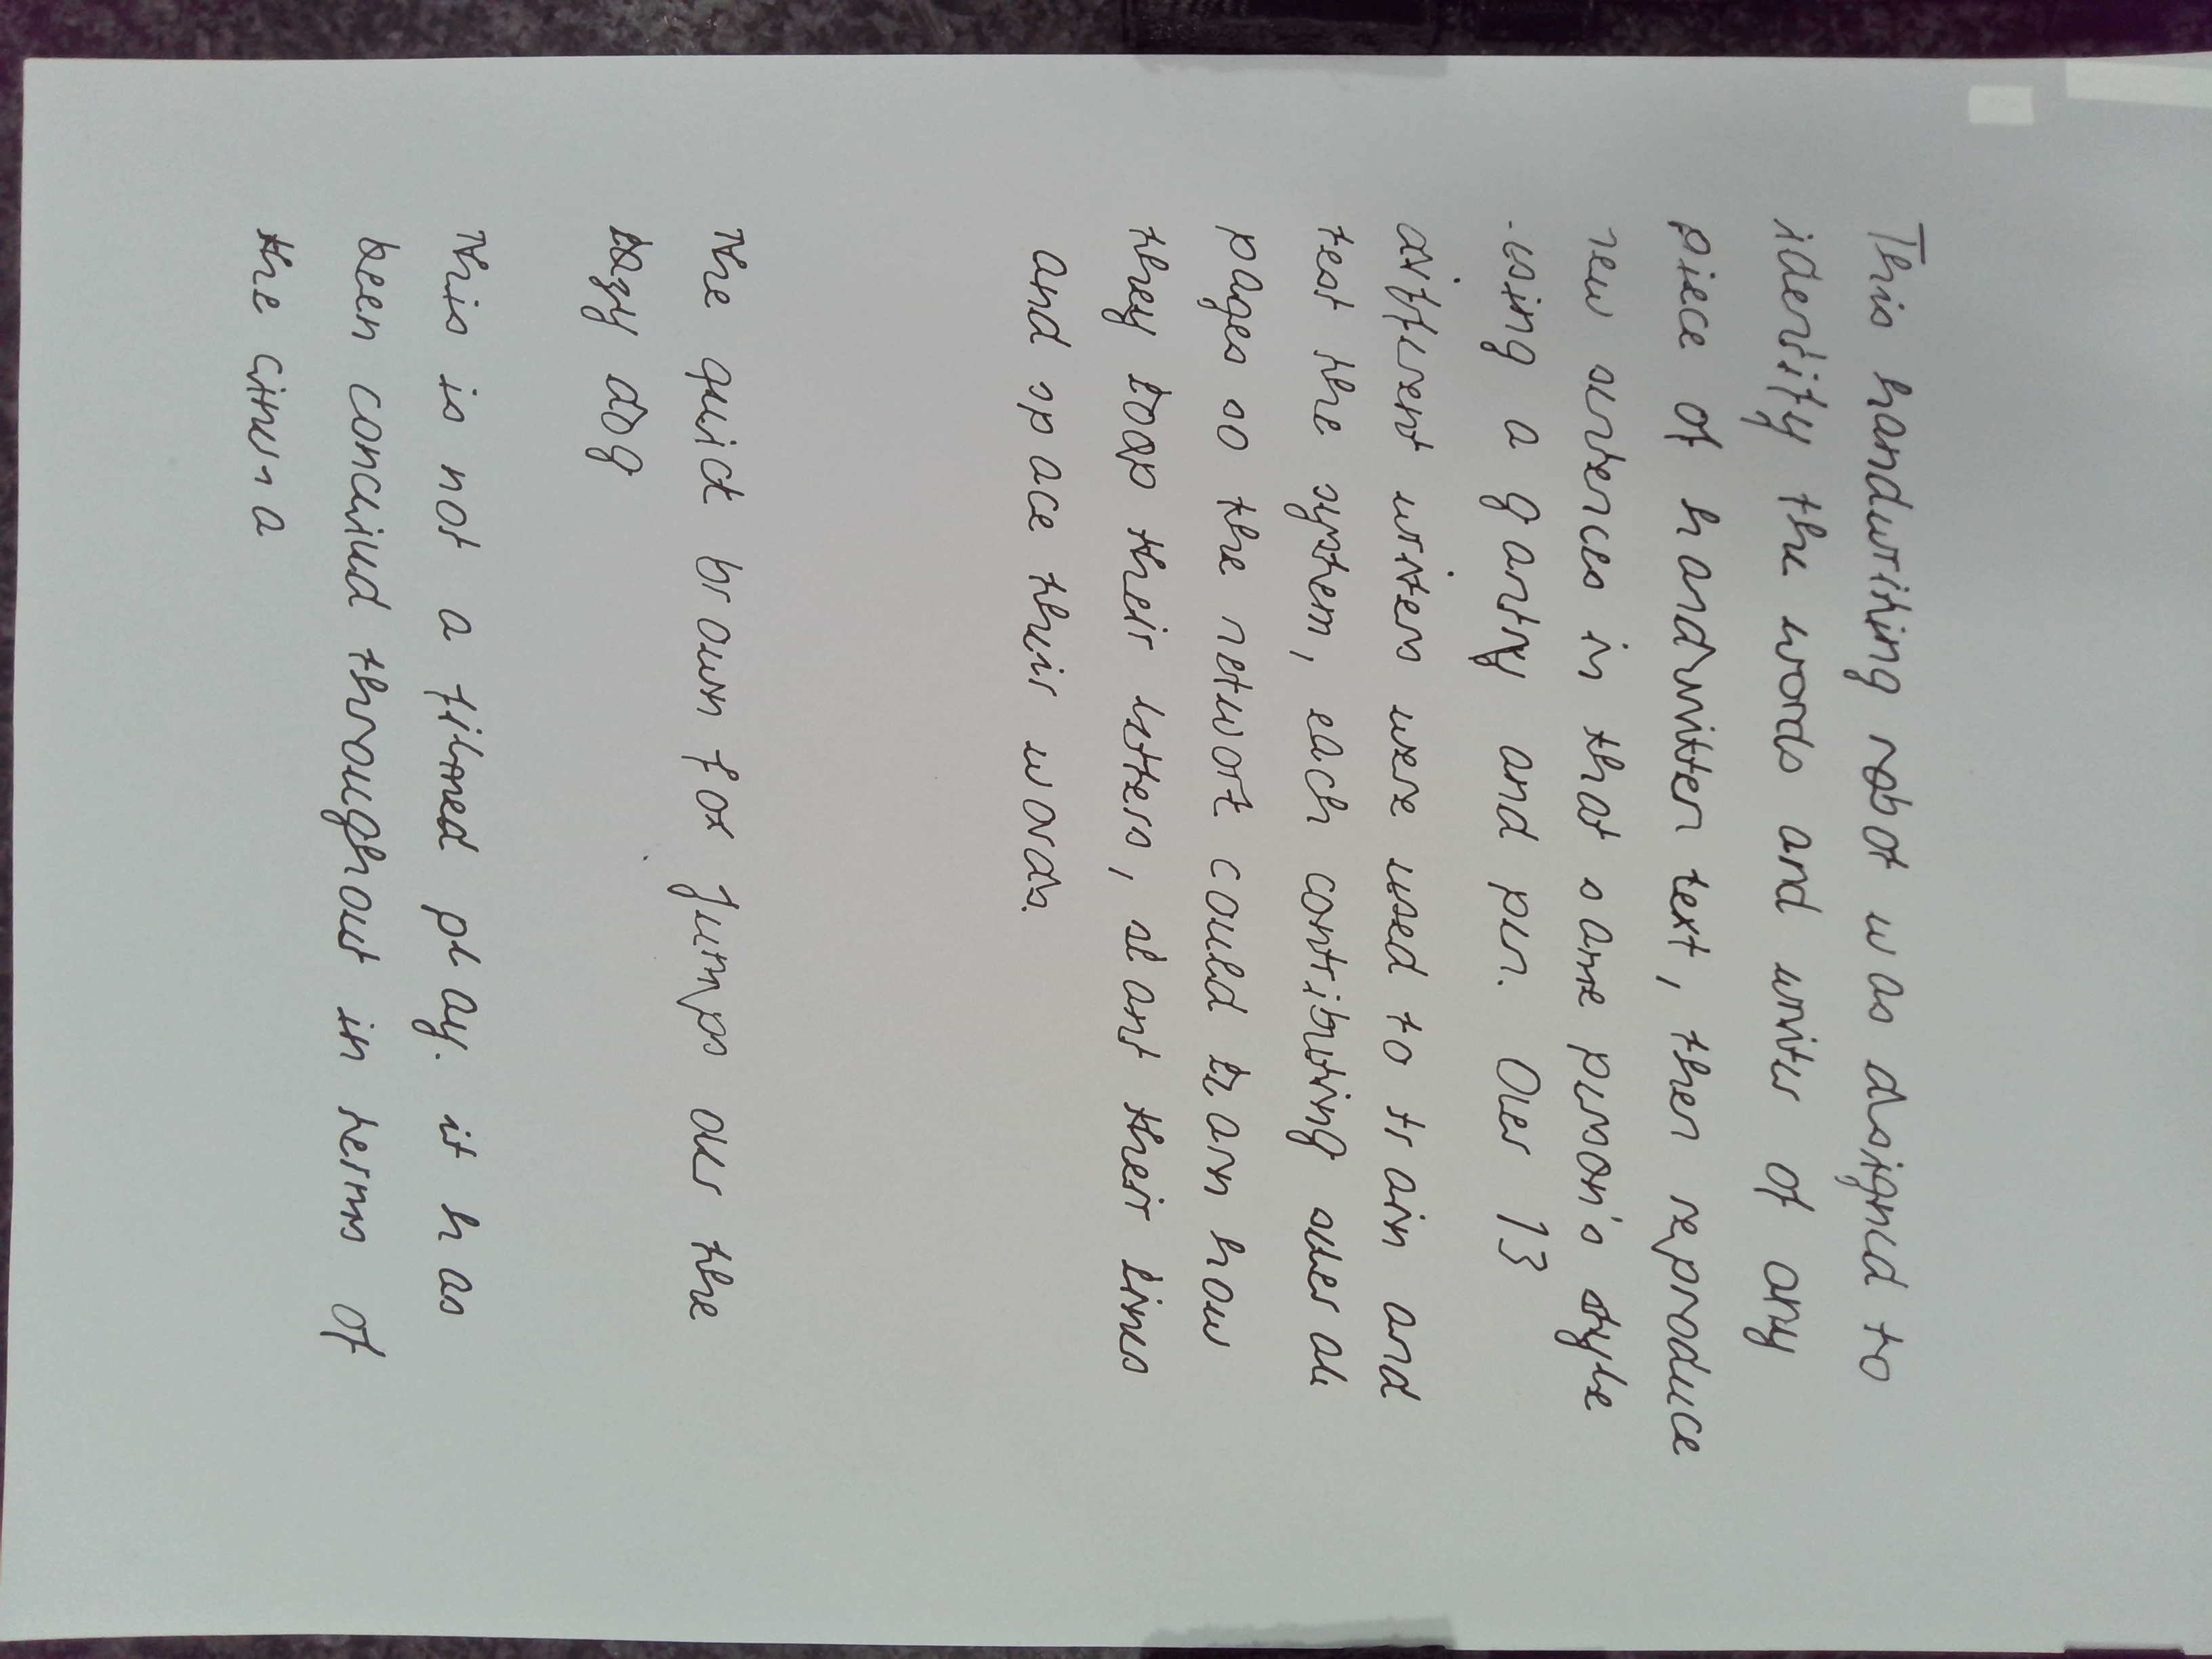
\includegraphics[angle=90,width=\linewidth,height=.55\textheight,keepaspectratio]{Figures/PhysicalPages/Author152.jpg}\par Author152\end{minipage}\hfill
\caption{Physical pages Author150, Author152.}\label{fig:app-physical-pages-1}\end{figure}\FloatBarrier

Figure~\ref{fig:app-physical-pages-2} preserves the photographed pages Author1531, Author1532. The scores come from their paired line records, not a visual estimate.
\begin{figure}[!htbp]\centering
\begin{minipage}{.48\linewidth}\centering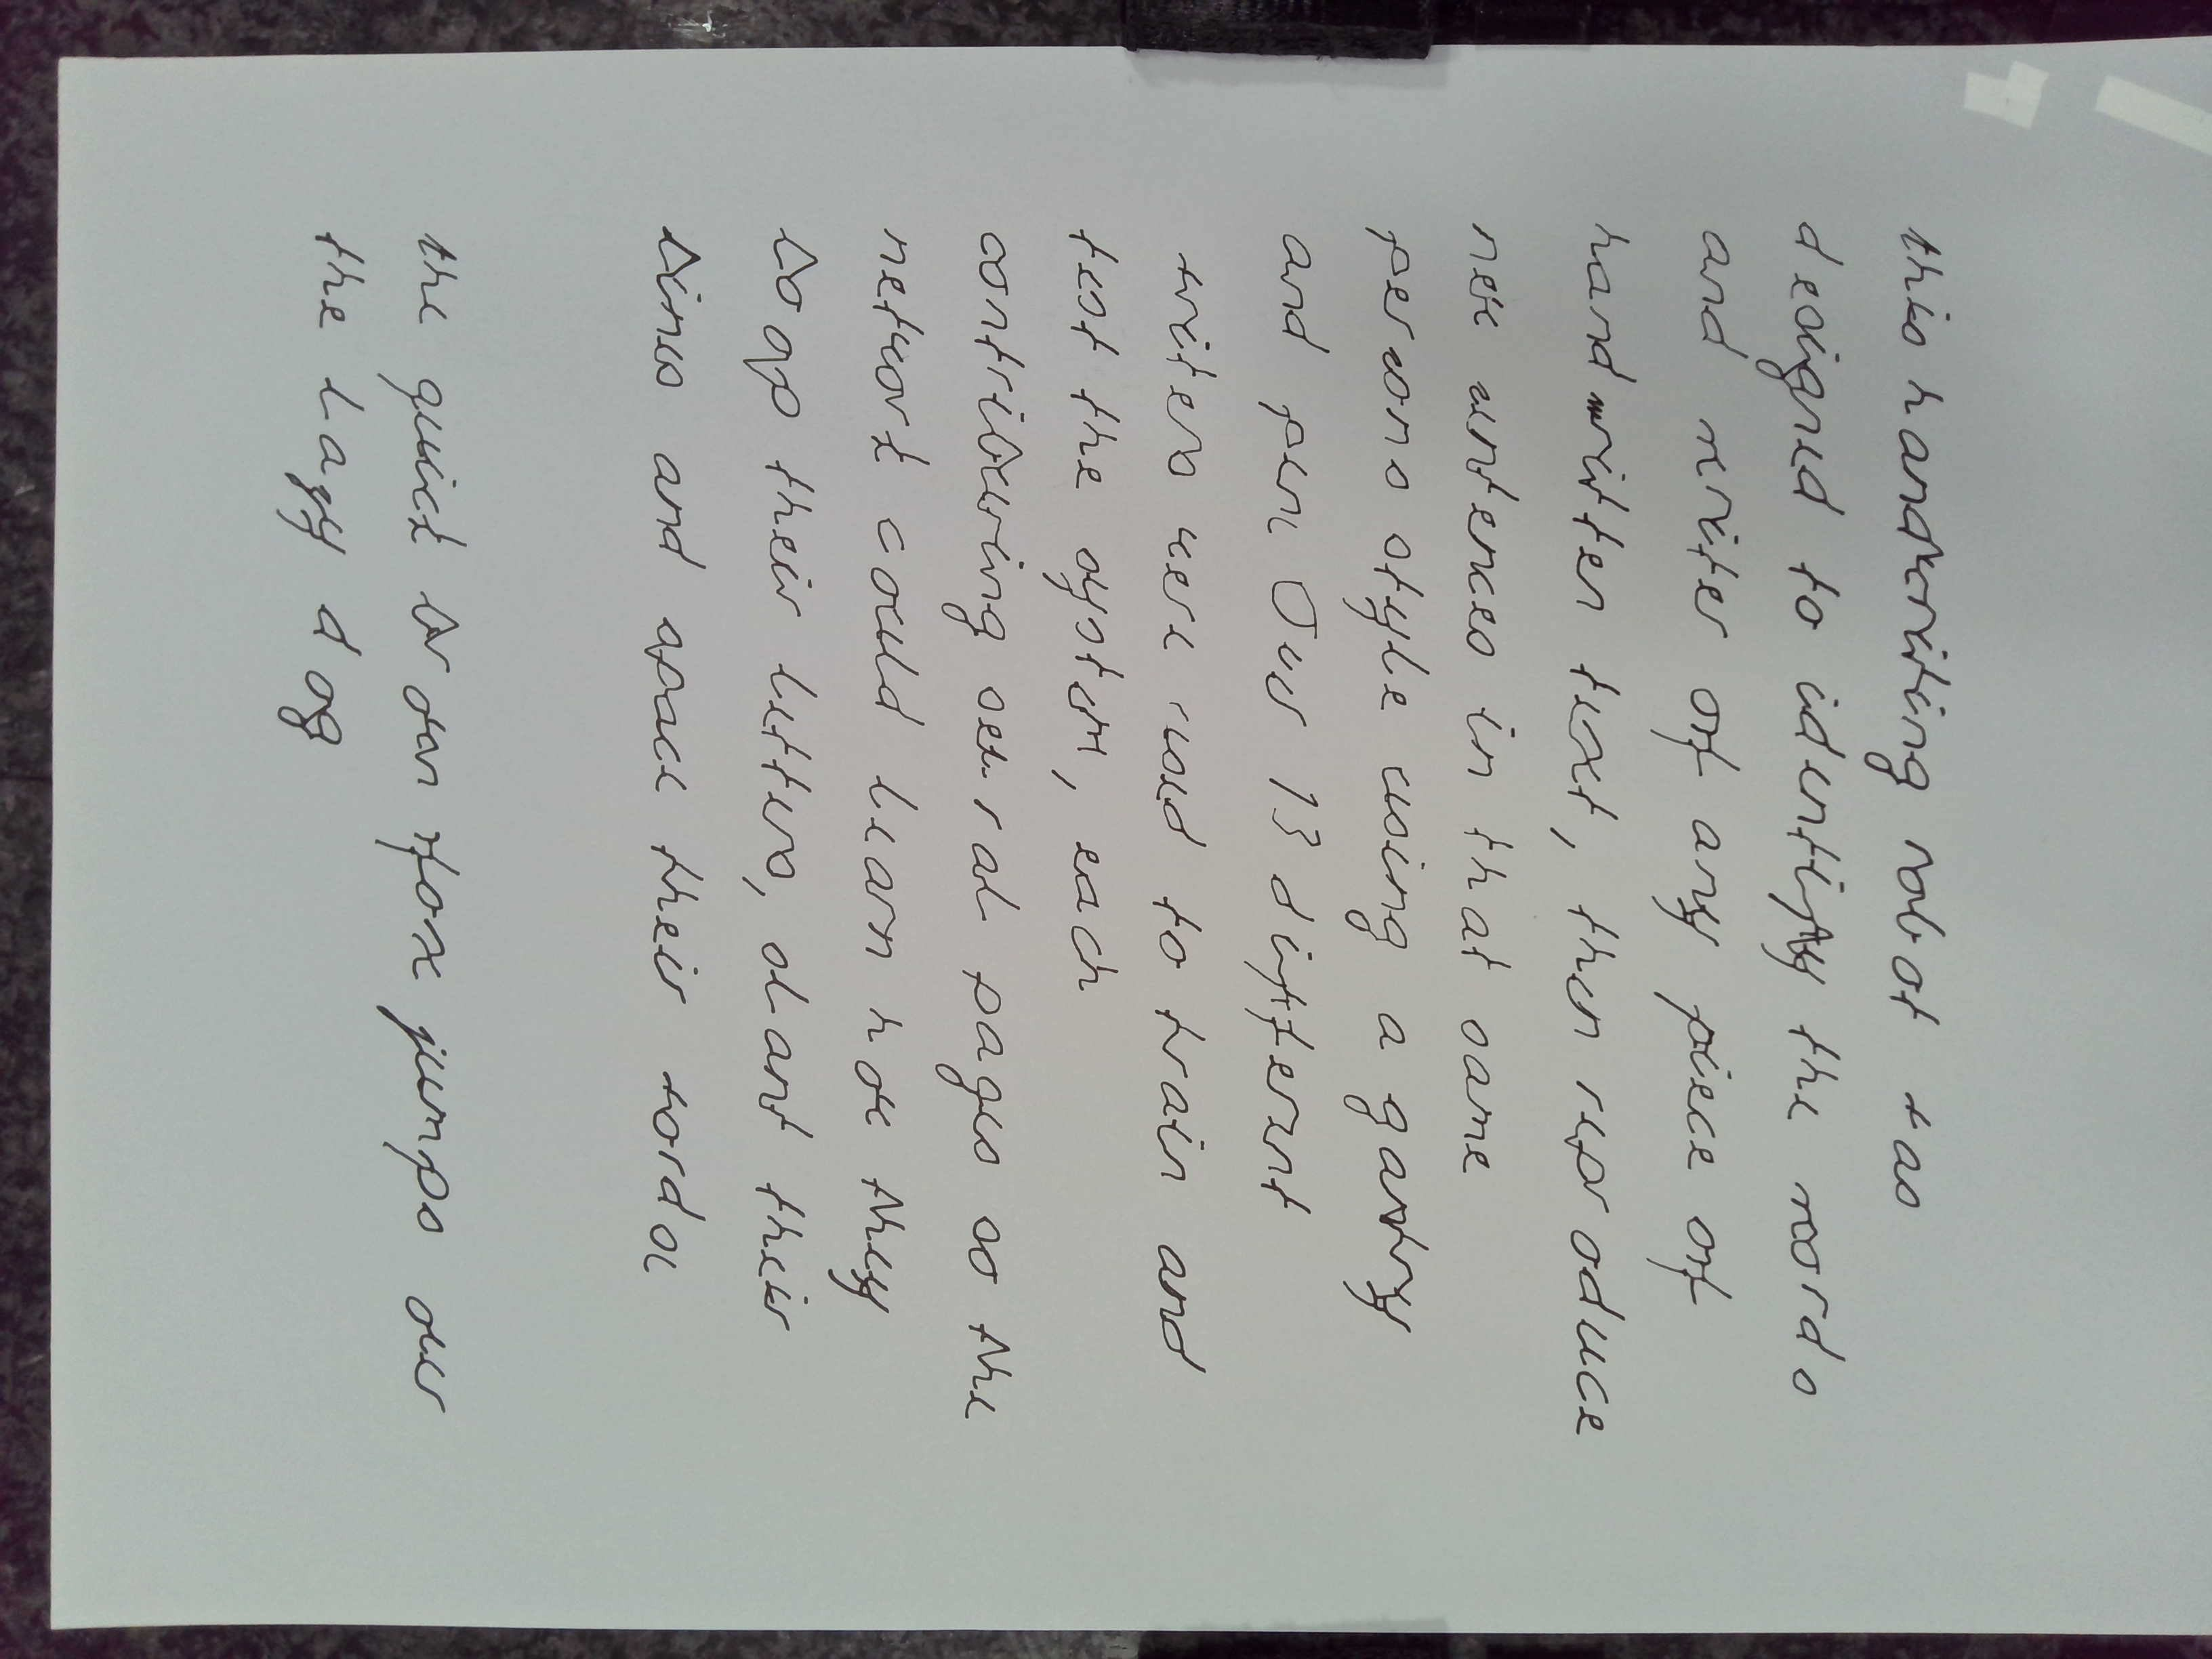
\includegraphics[angle=90,width=\linewidth,height=.55\textheight,keepaspectratio]{Figures/PhysicalPages/Author1531.jpg}\par Author1531\end{minipage}\hfill
\begin{minipage}{.48\linewidth}\centering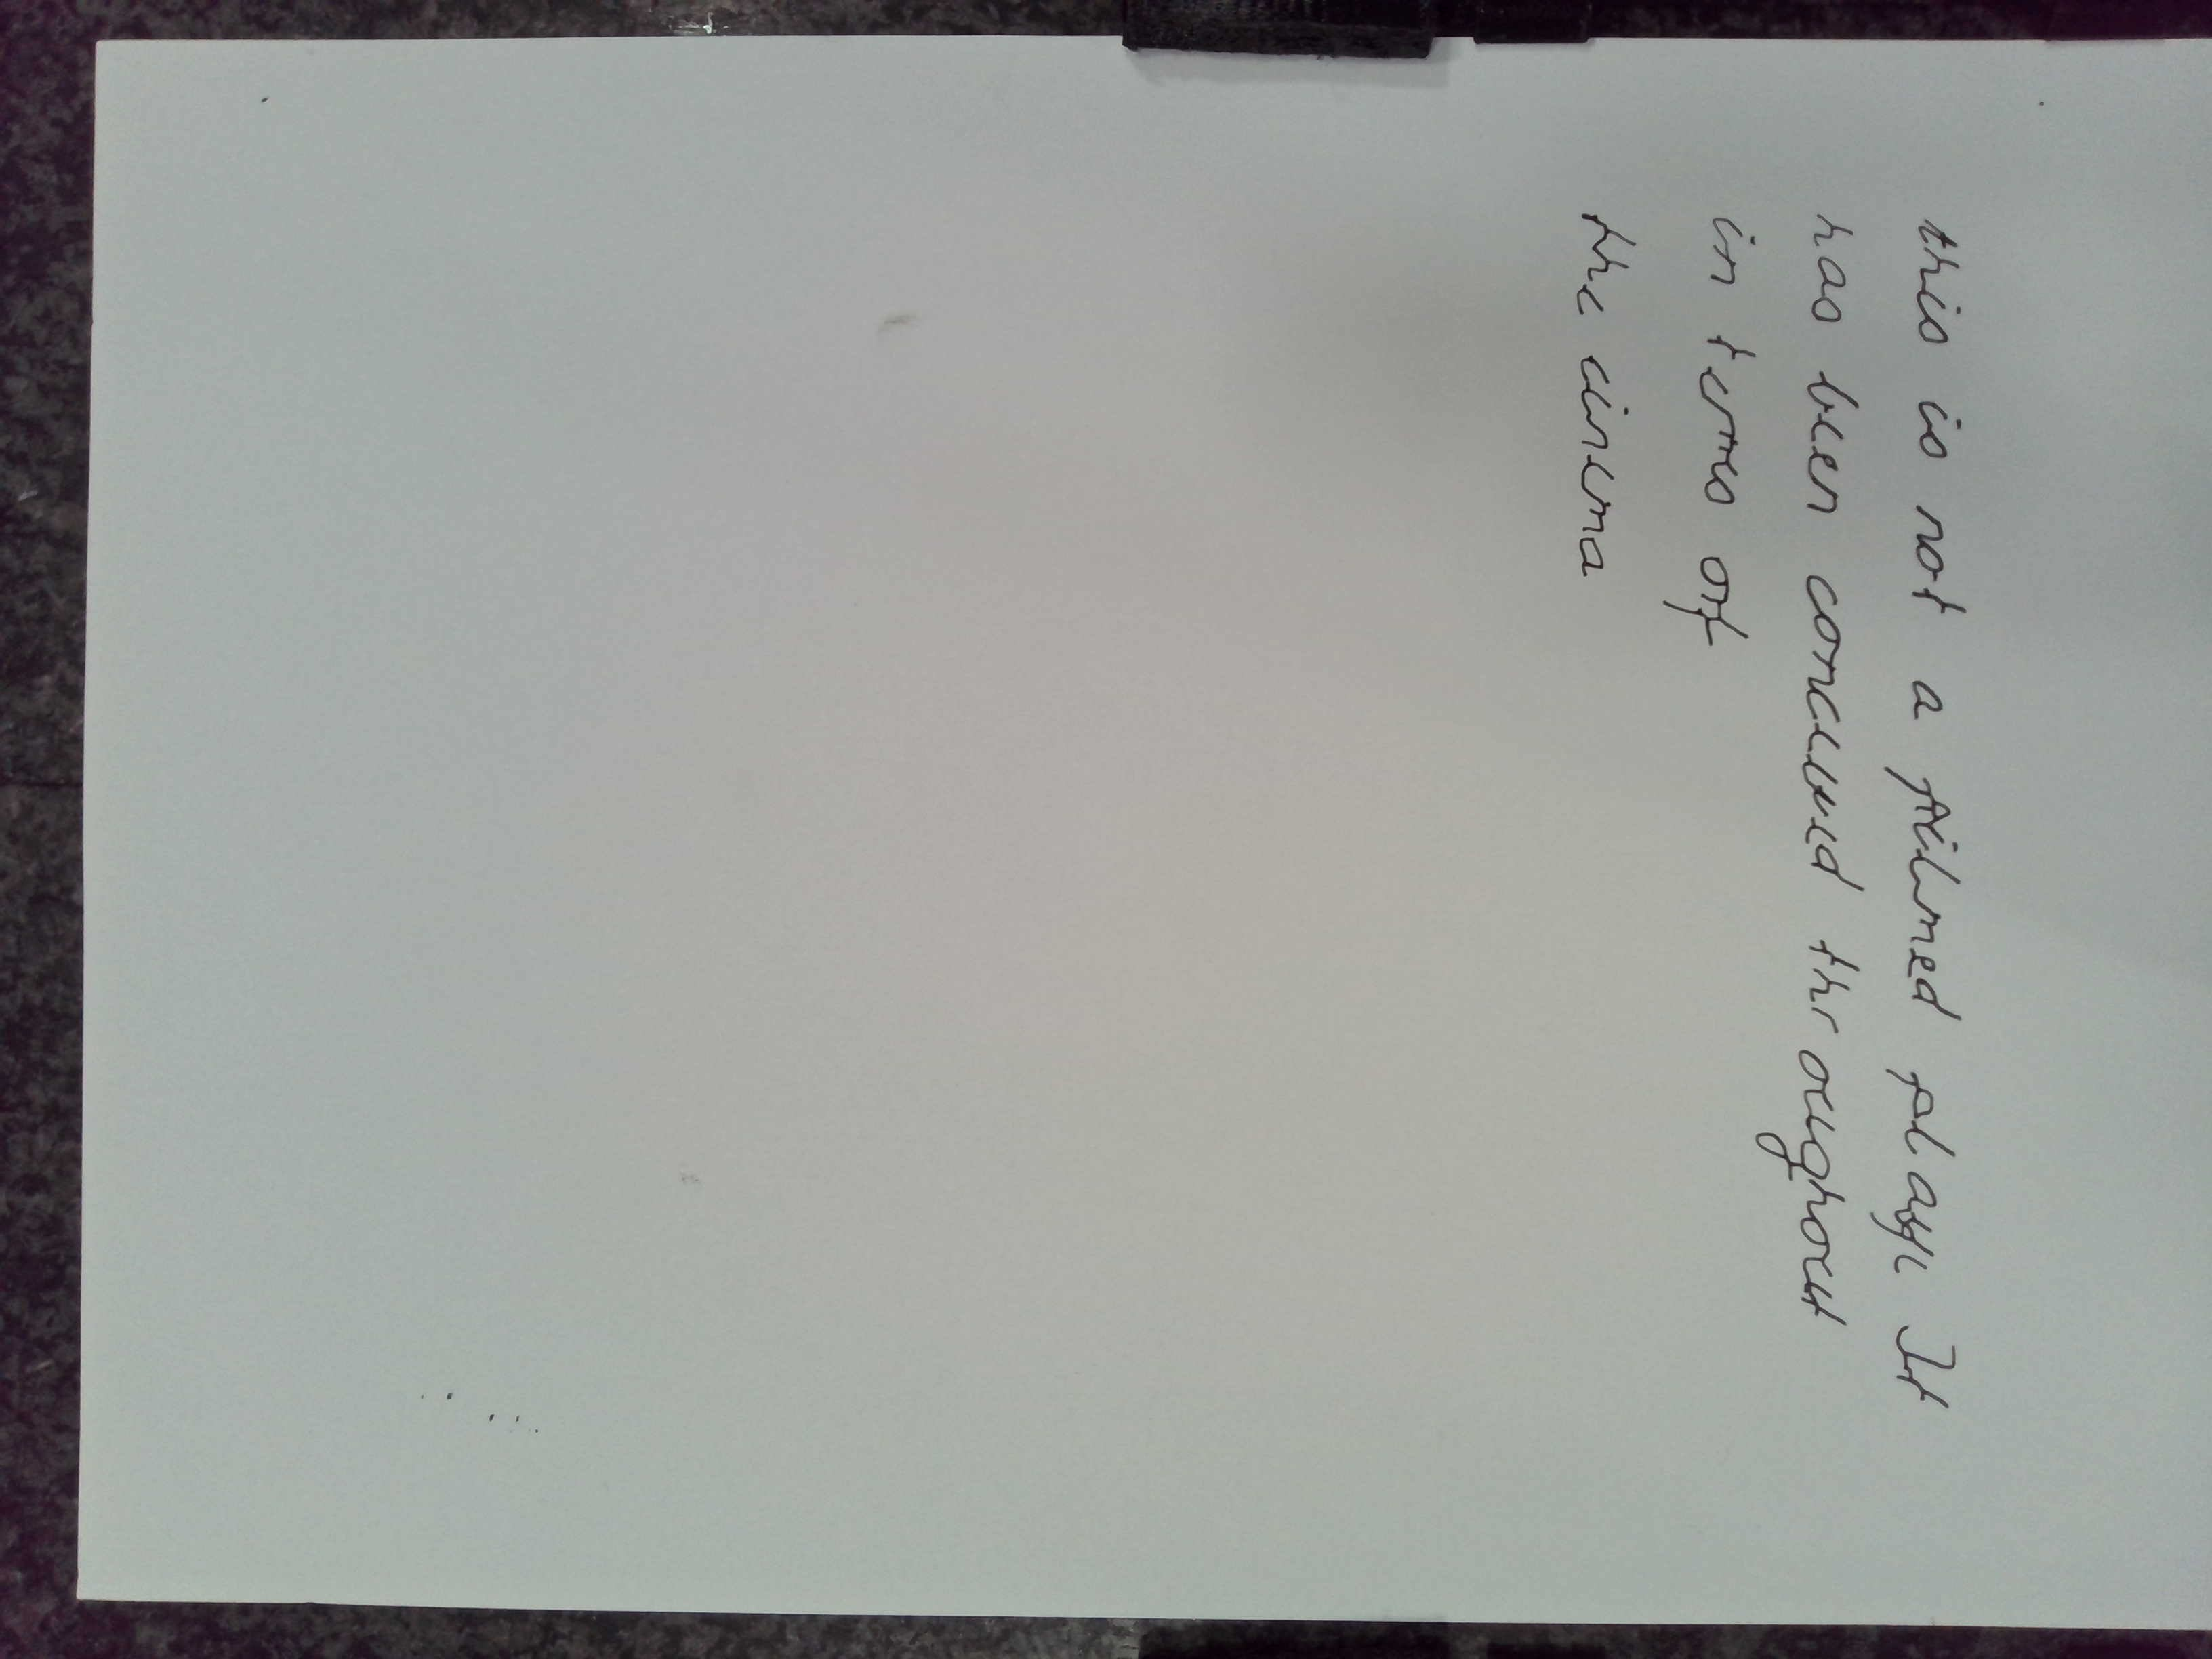
\includegraphics[angle=90,width=\linewidth,height=.55\textheight,keepaspectratio]{Figures/PhysicalPages/Author1532.jpg}\par Author1532\end{minipage}\hfill
\caption{Physical pages Author1531, Author1532.}\label{fig:app-physical-pages-2}\end{figure}\FloatBarrier

Figure~\ref{fig:app-physical-pages-3} preserves the photographed pages Author3841, Author3842. The scores come from their paired line records, not a visual estimate.
\begin{figure}[!htbp]\centering
\begin{minipage}{.48\linewidth}\centering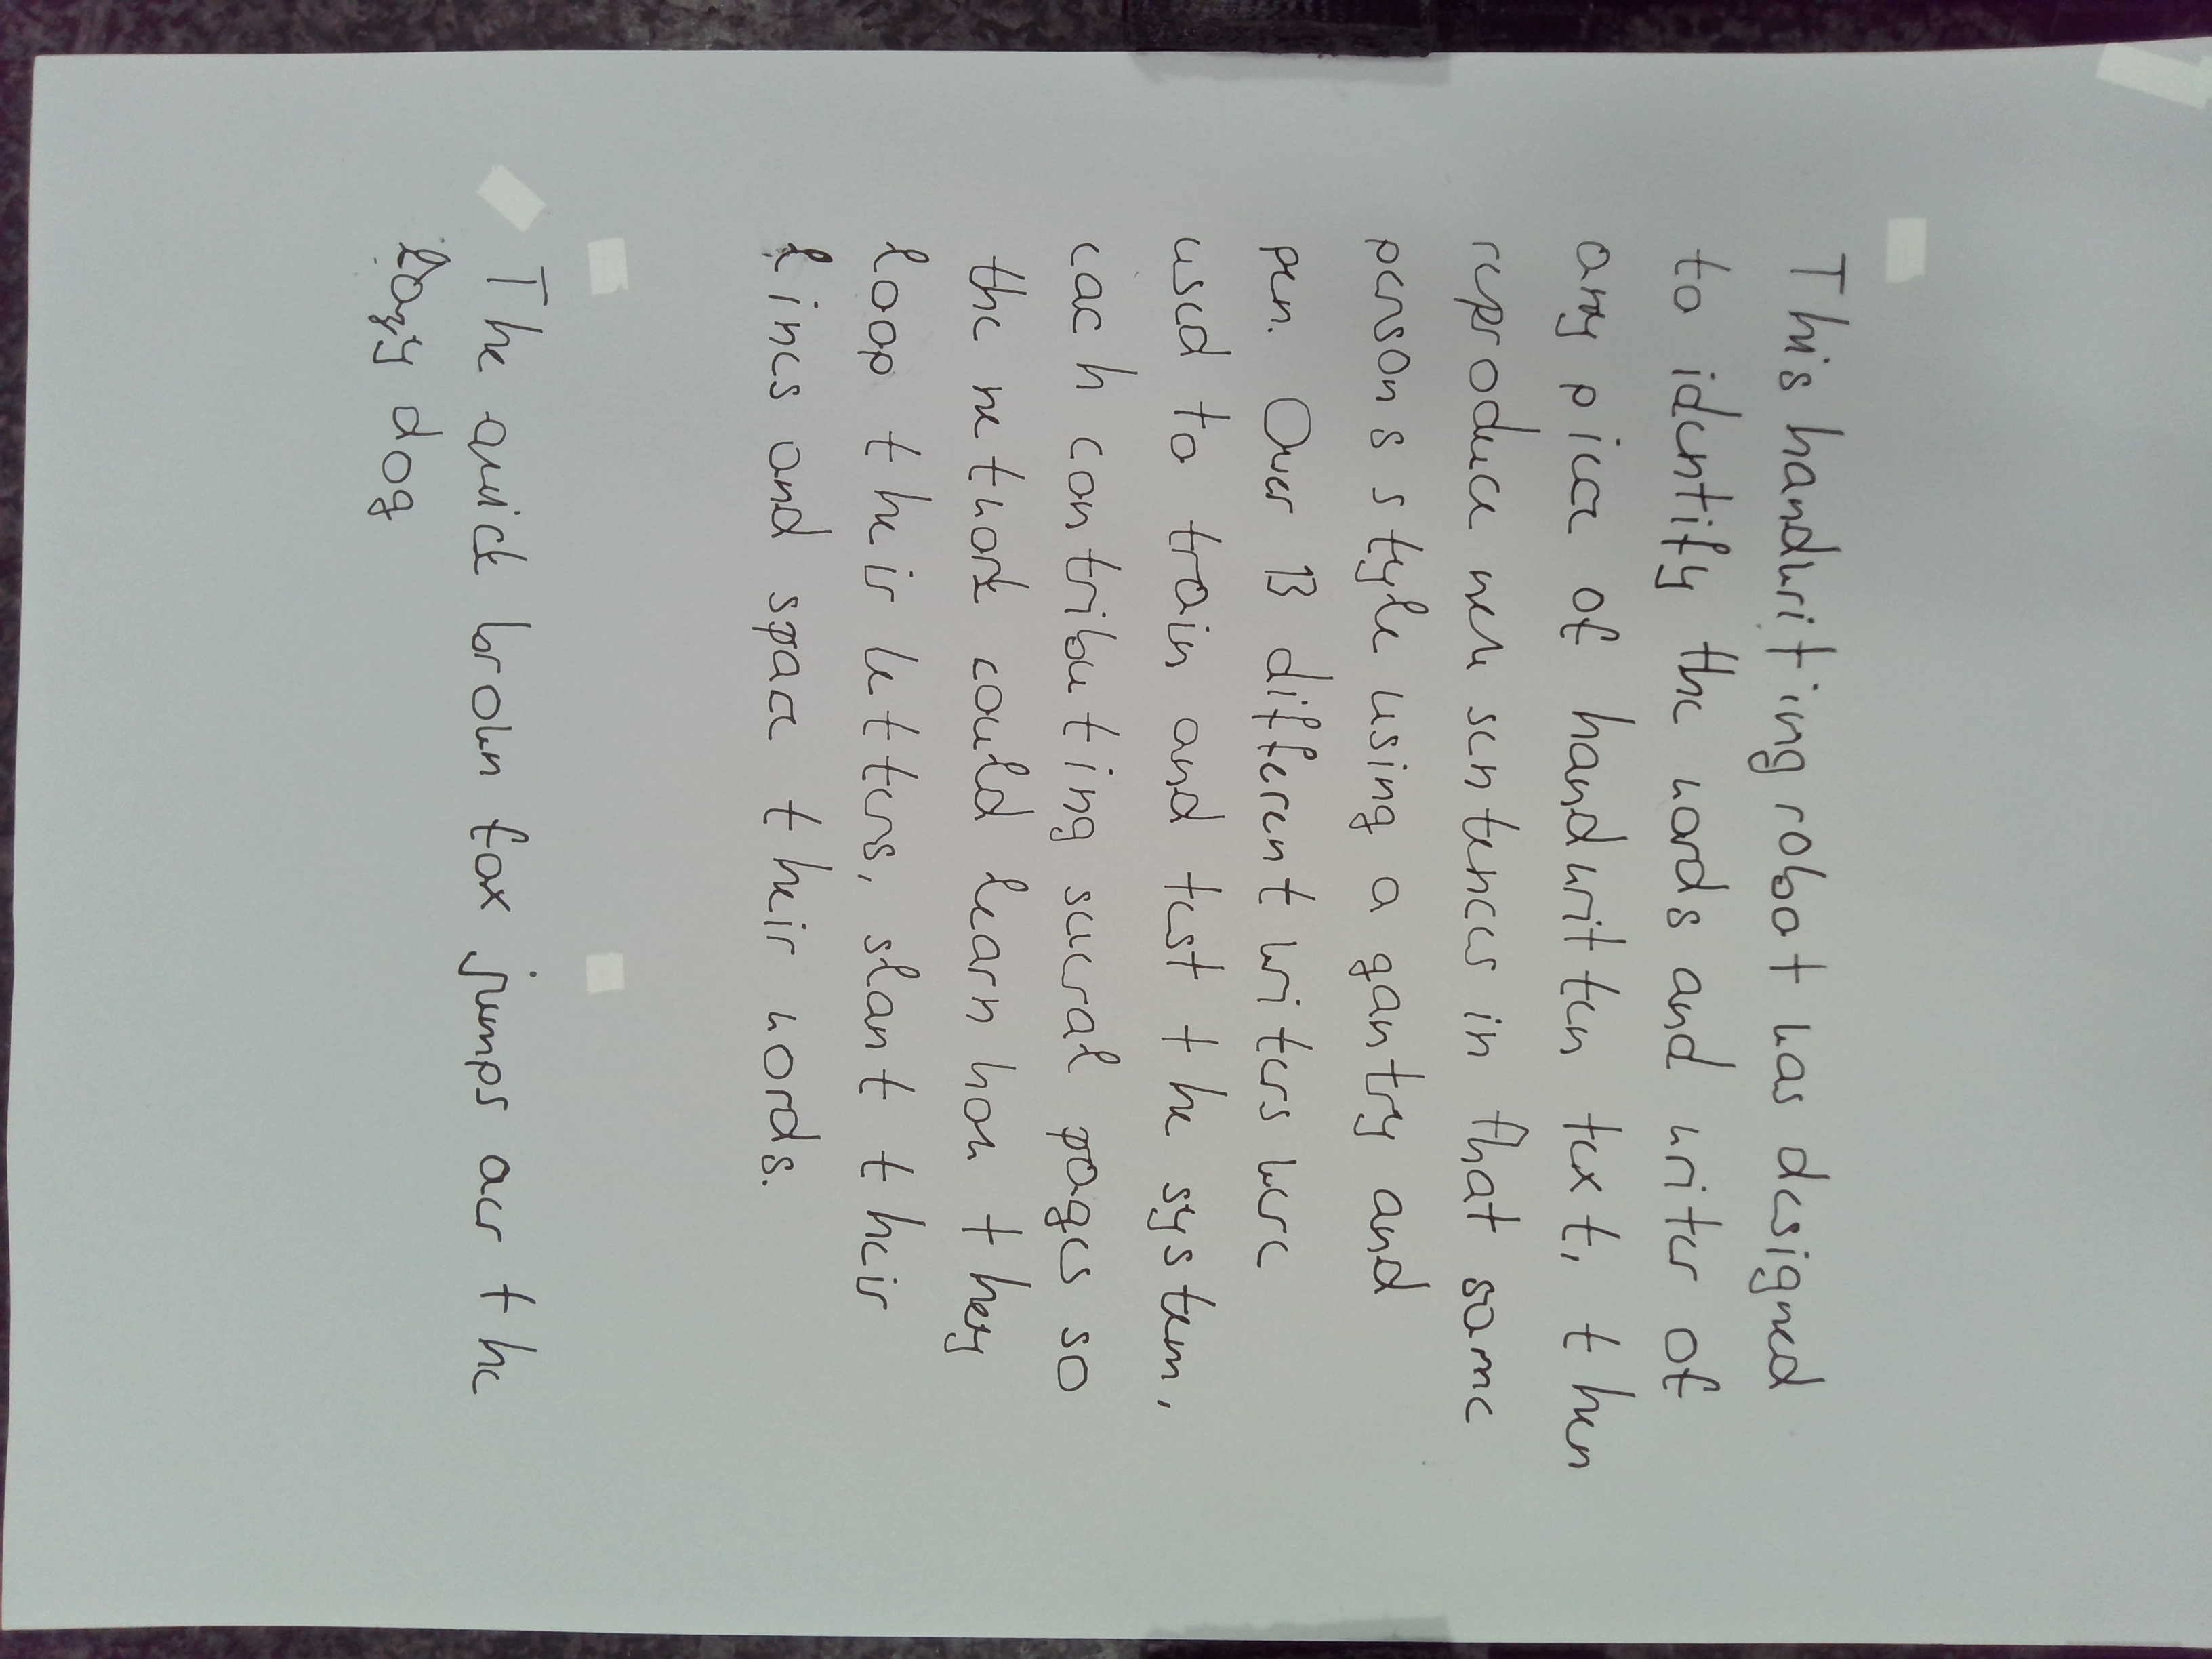
\includegraphics[angle=90,width=\linewidth,height=.55\textheight,keepaspectratio]{Figures/PhysicalPages/Author3841.jpg}\par Author3841\end{minipage}\hfill
\begin{minipage}{.48\linewidth}\centering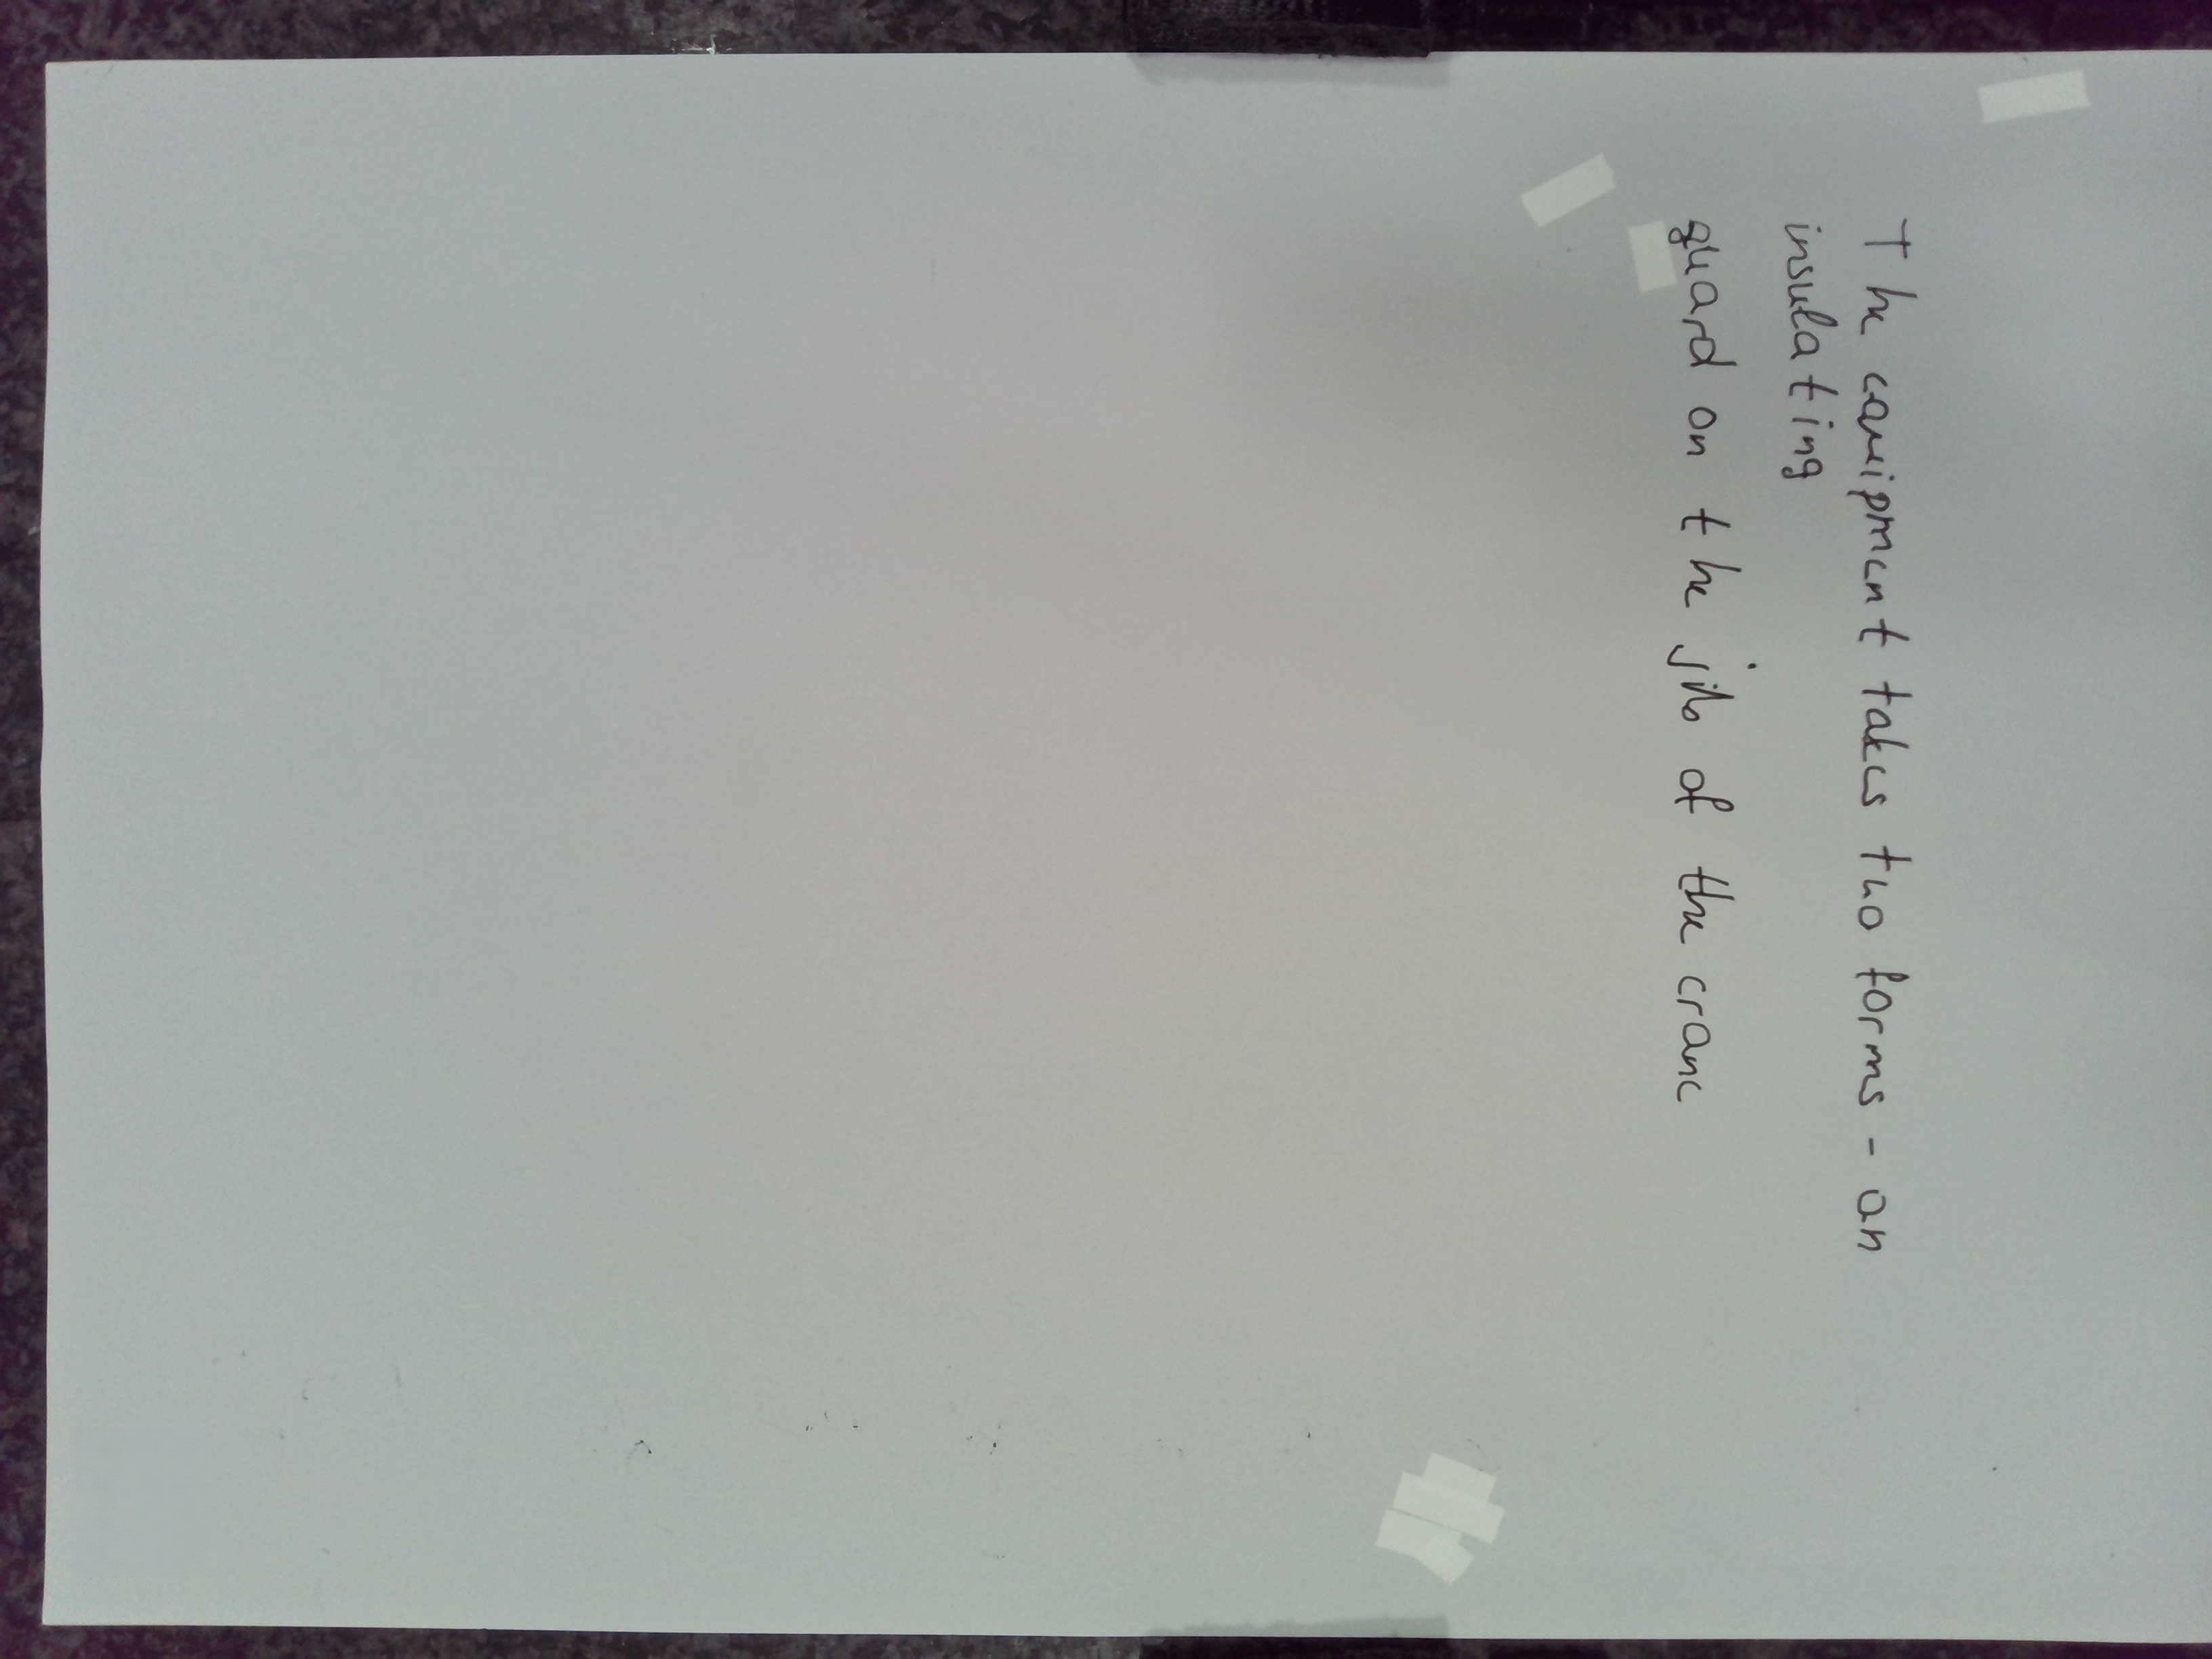
\includegraphics[angle=90,width=\linewidth,height=.55\textheight,keepaspectratio]{Figures/PhysicalPages/Author3842.jpg}\par Author3842\end{minipage}\hfill
\caption{Physical pages Author3841, Author3842.}\label{fig:app-physical-pages-3}\end{figure}\FloatBarrier

Figure~\ref{fig:app-physical-pages-4} preserves the photographed pages Author552, Author588. The scores come from their paired line records, not a visual estimate.
\begin{figure}[!htbp]\centering
\begin{minipage}{.48\linewidth}\centering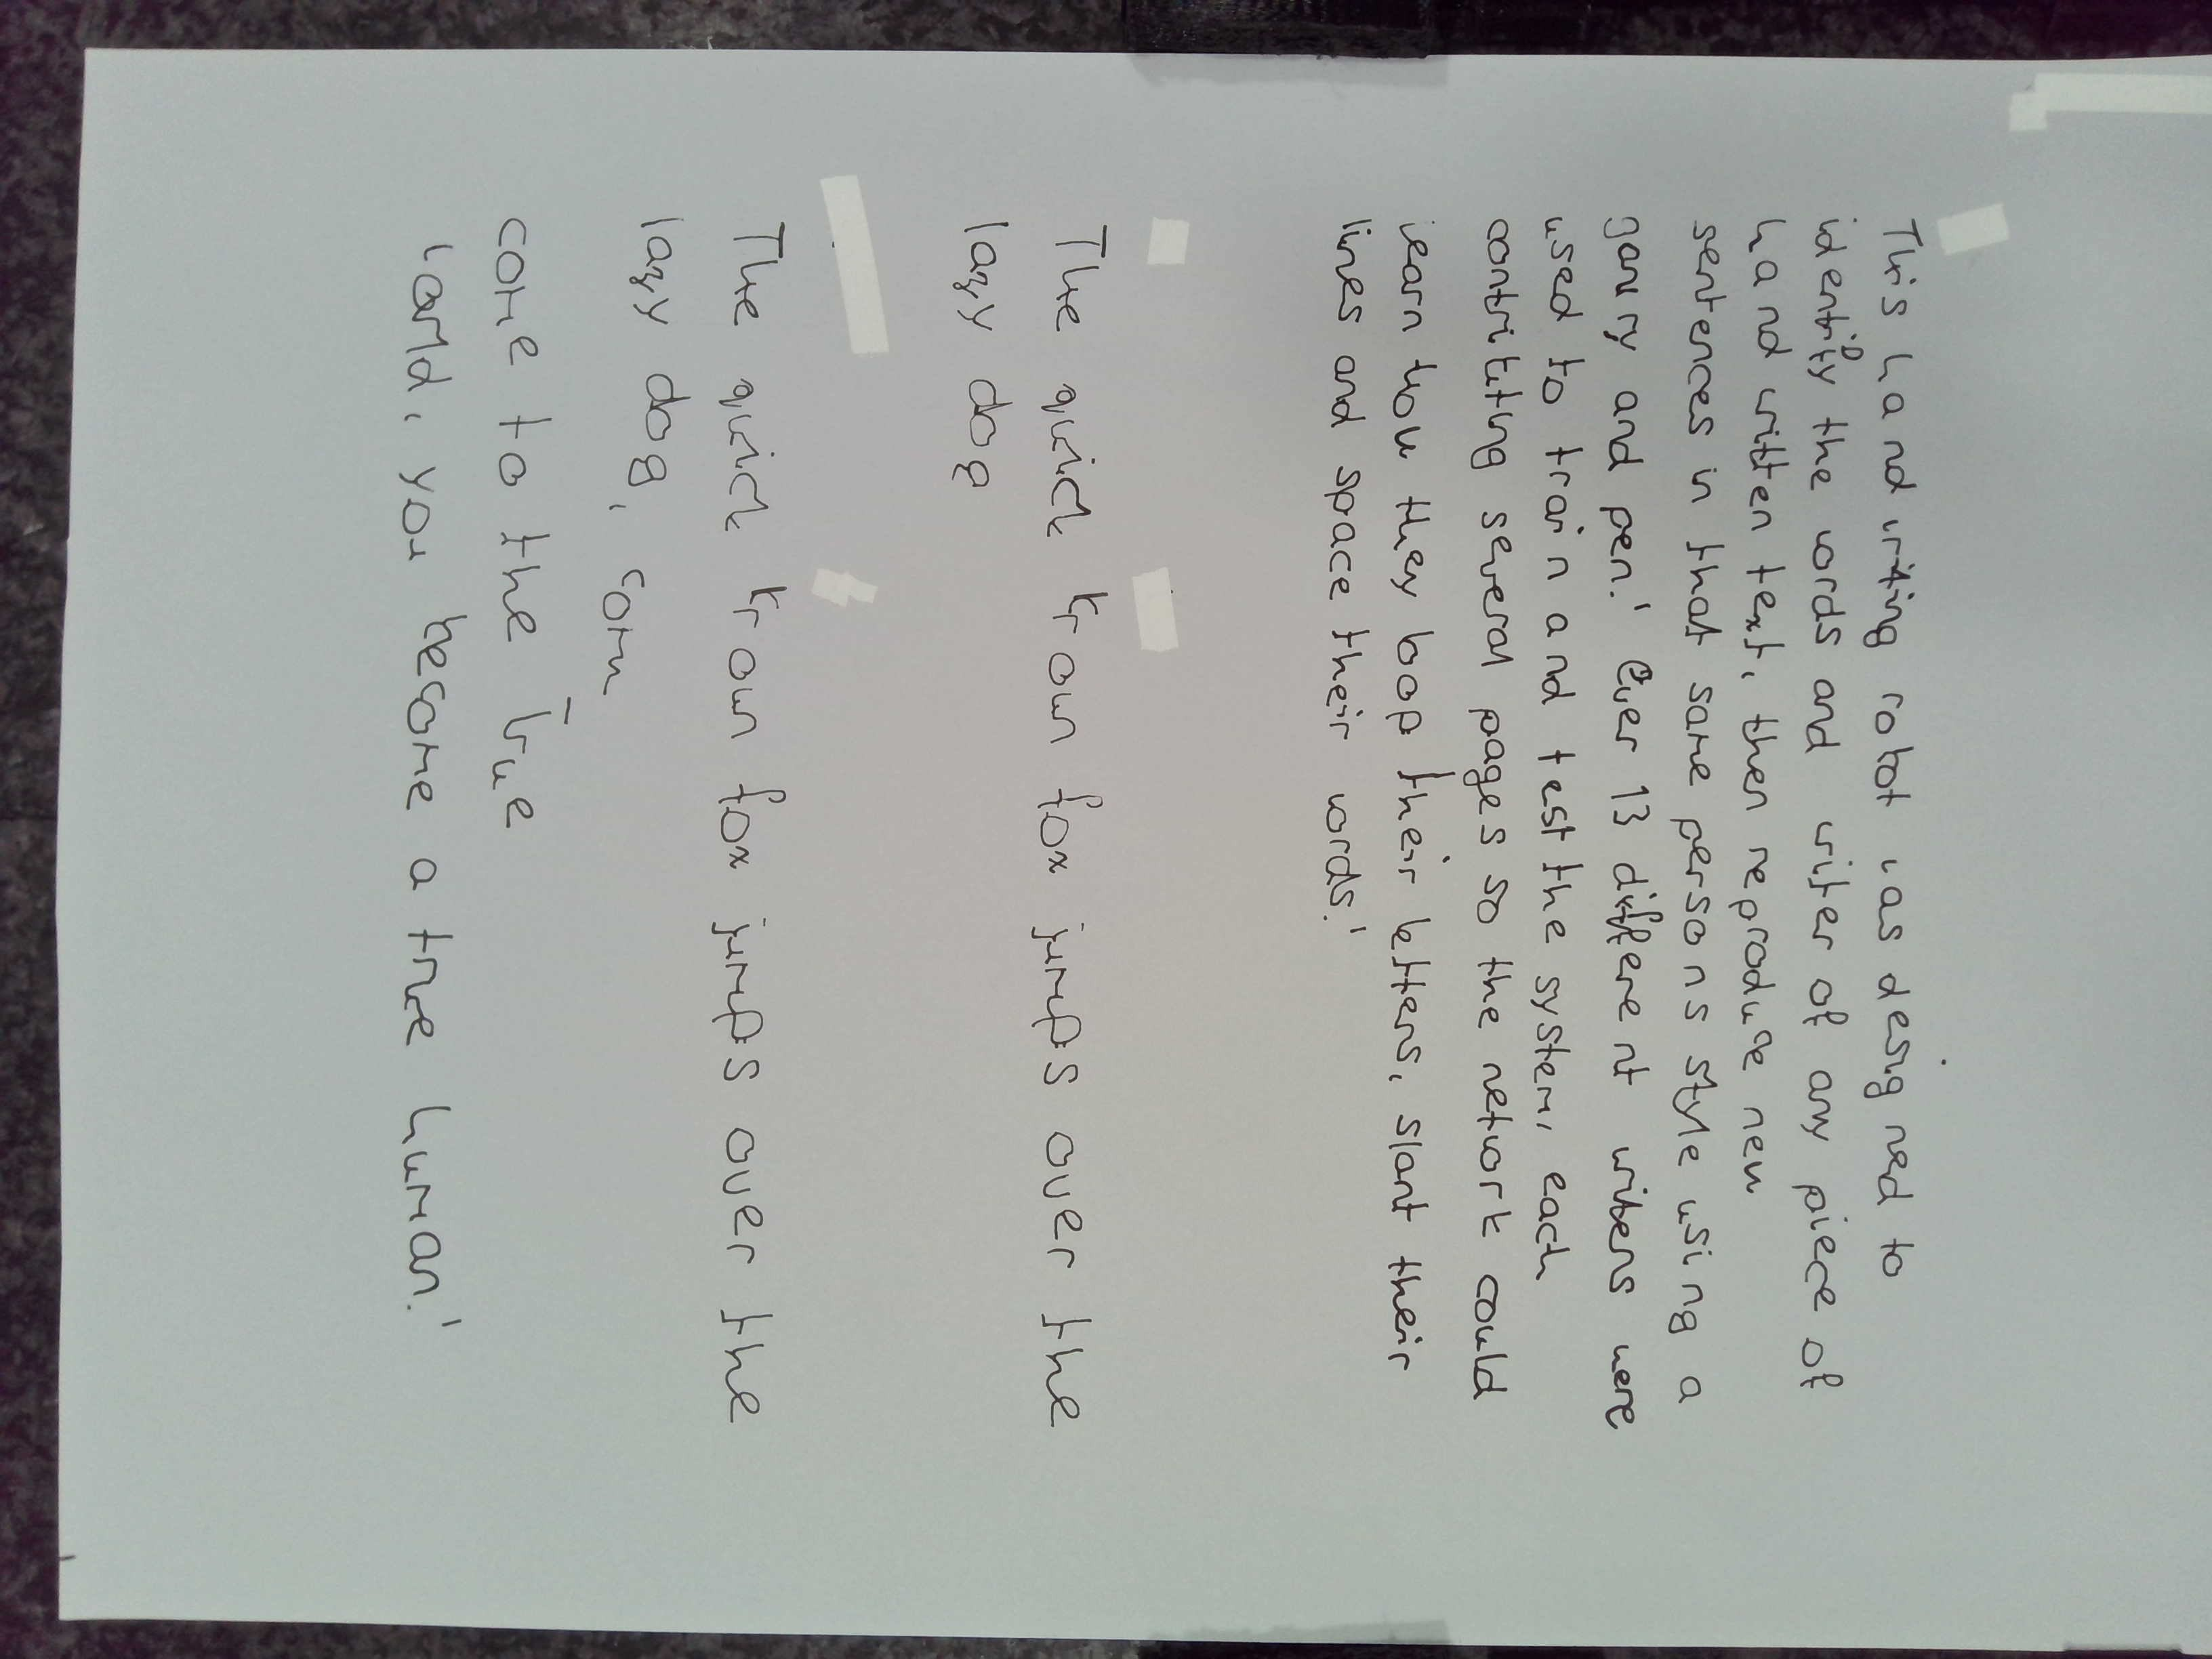
\includegraphics[angle=90,width=\linewidth,height=.55\textheight,keepaspectratio]{Figures/PhysicalPages/Author552.jpg}\par Author552\end{minipage}\hfill
\begin{minipage}{.48\linewidth}\centering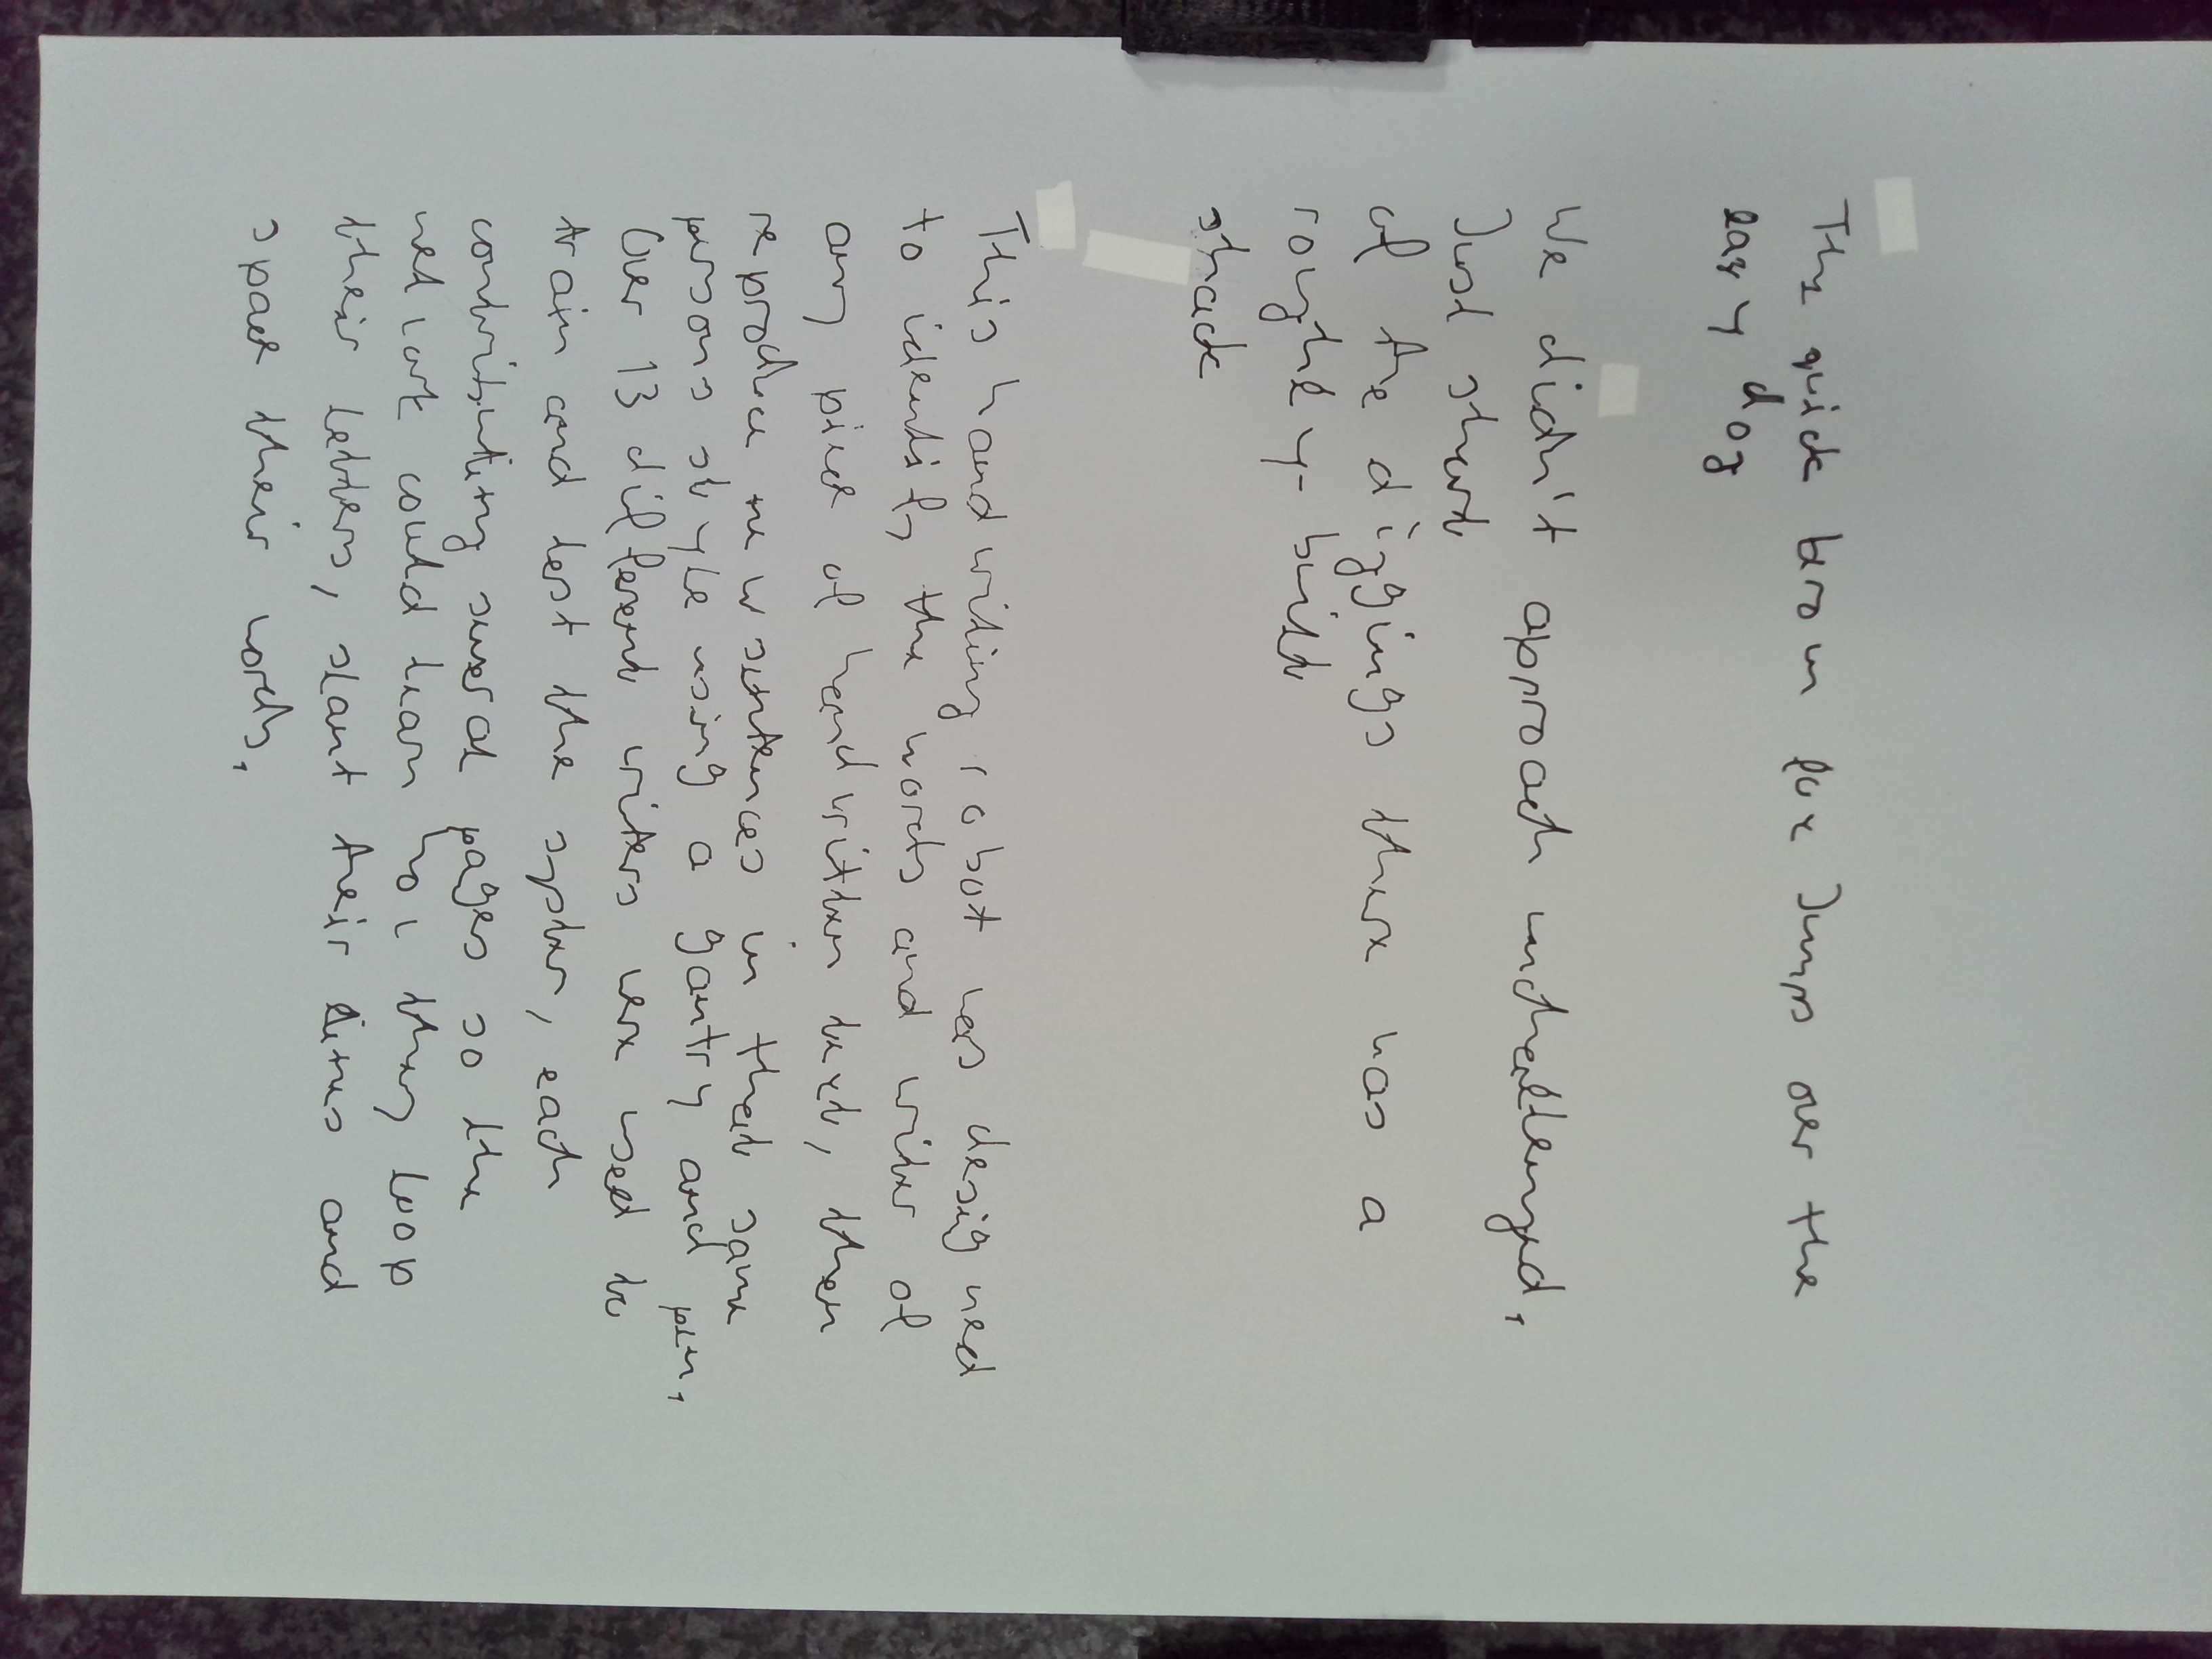
\includegraphics[angle=90,width=\linewidth,height=.55\textheight,keepaspectratio]{Figures/PhysicalPages/Author588.jpg}\par Author588\end{minipage}\hfill
\caption{Physical pages Author552, Author588.}\label{fig:app-physical-pages-4}\end{figure}\FloatBarrier

Figure~\ref{fig:app-physical-pages-5} preserves the photographed pages AuthorA1, AuthorA2. The scores come from their paired line records, not a visual estimate.
\begin{figure}[!htbp]\centering
\begin{minipage}{.48\linewidth}\centering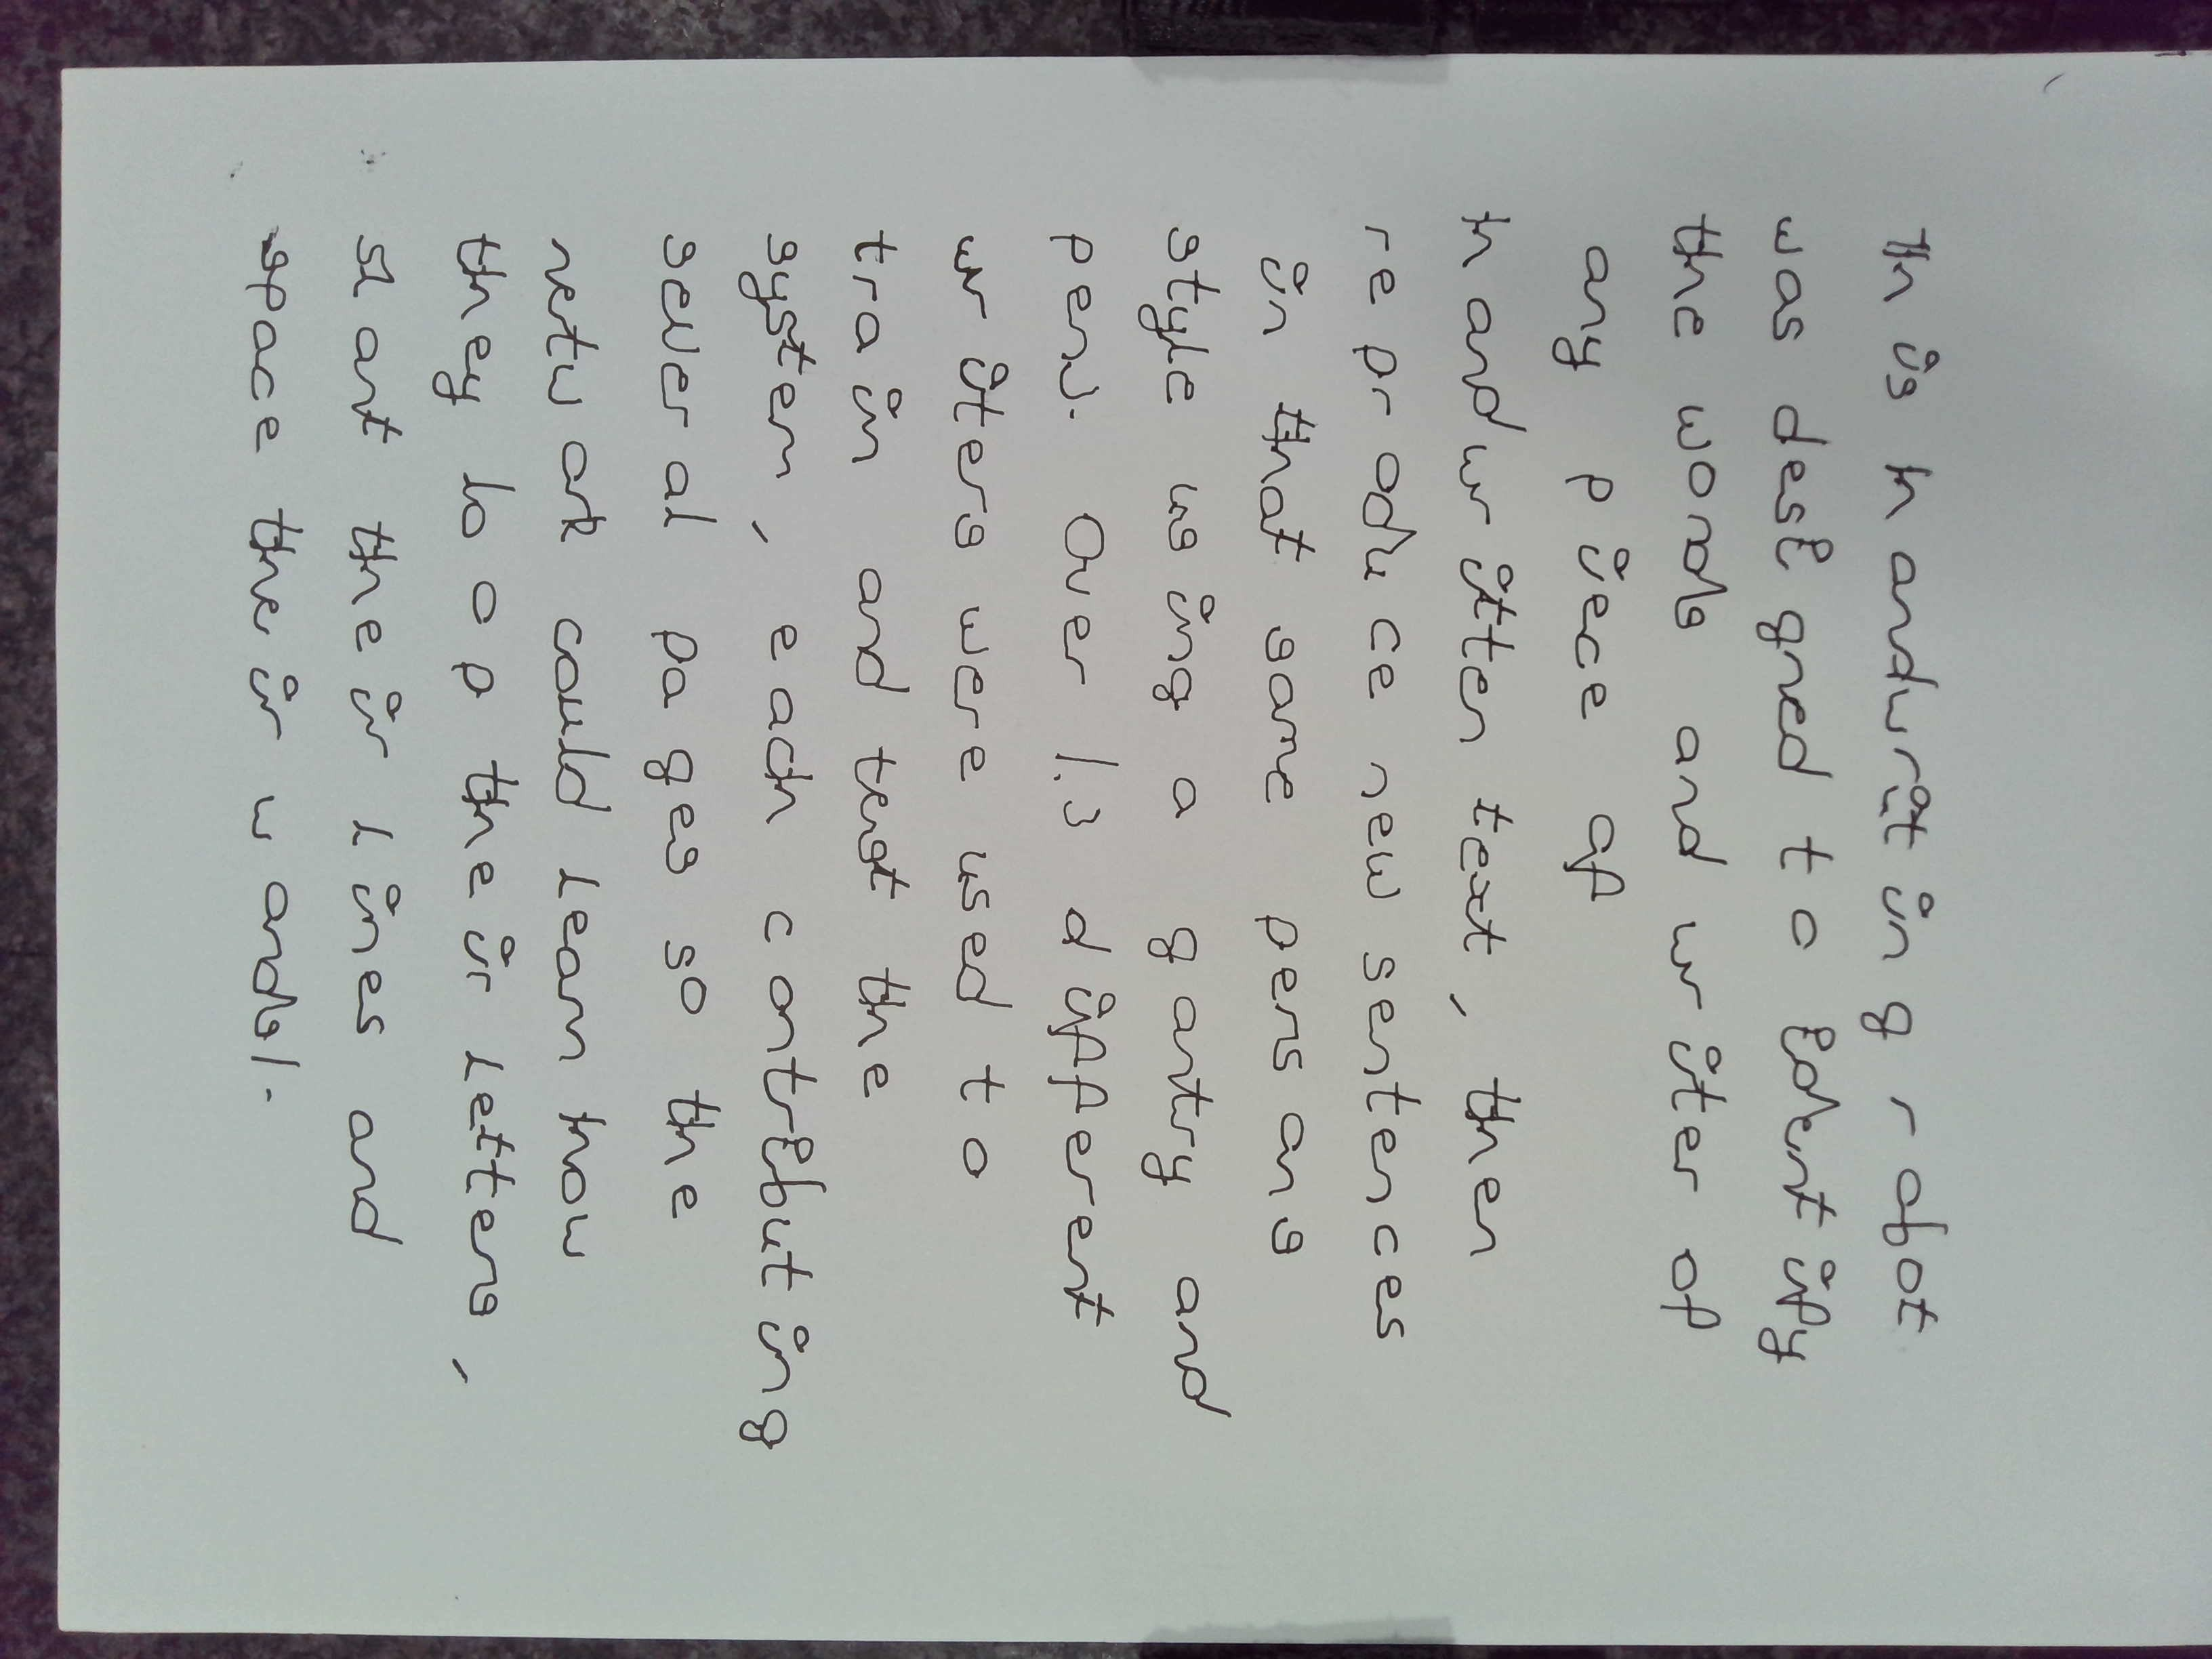
\includegraphics[angle=90,width=\linewidth,height=.55\textheight,keepaspectratio]{Figures/PhysicalPages/AuthorA1.jpg}\par AuthorA1\end{minipage}\hfill
\begin{minipage}{.48\linewidth}\centering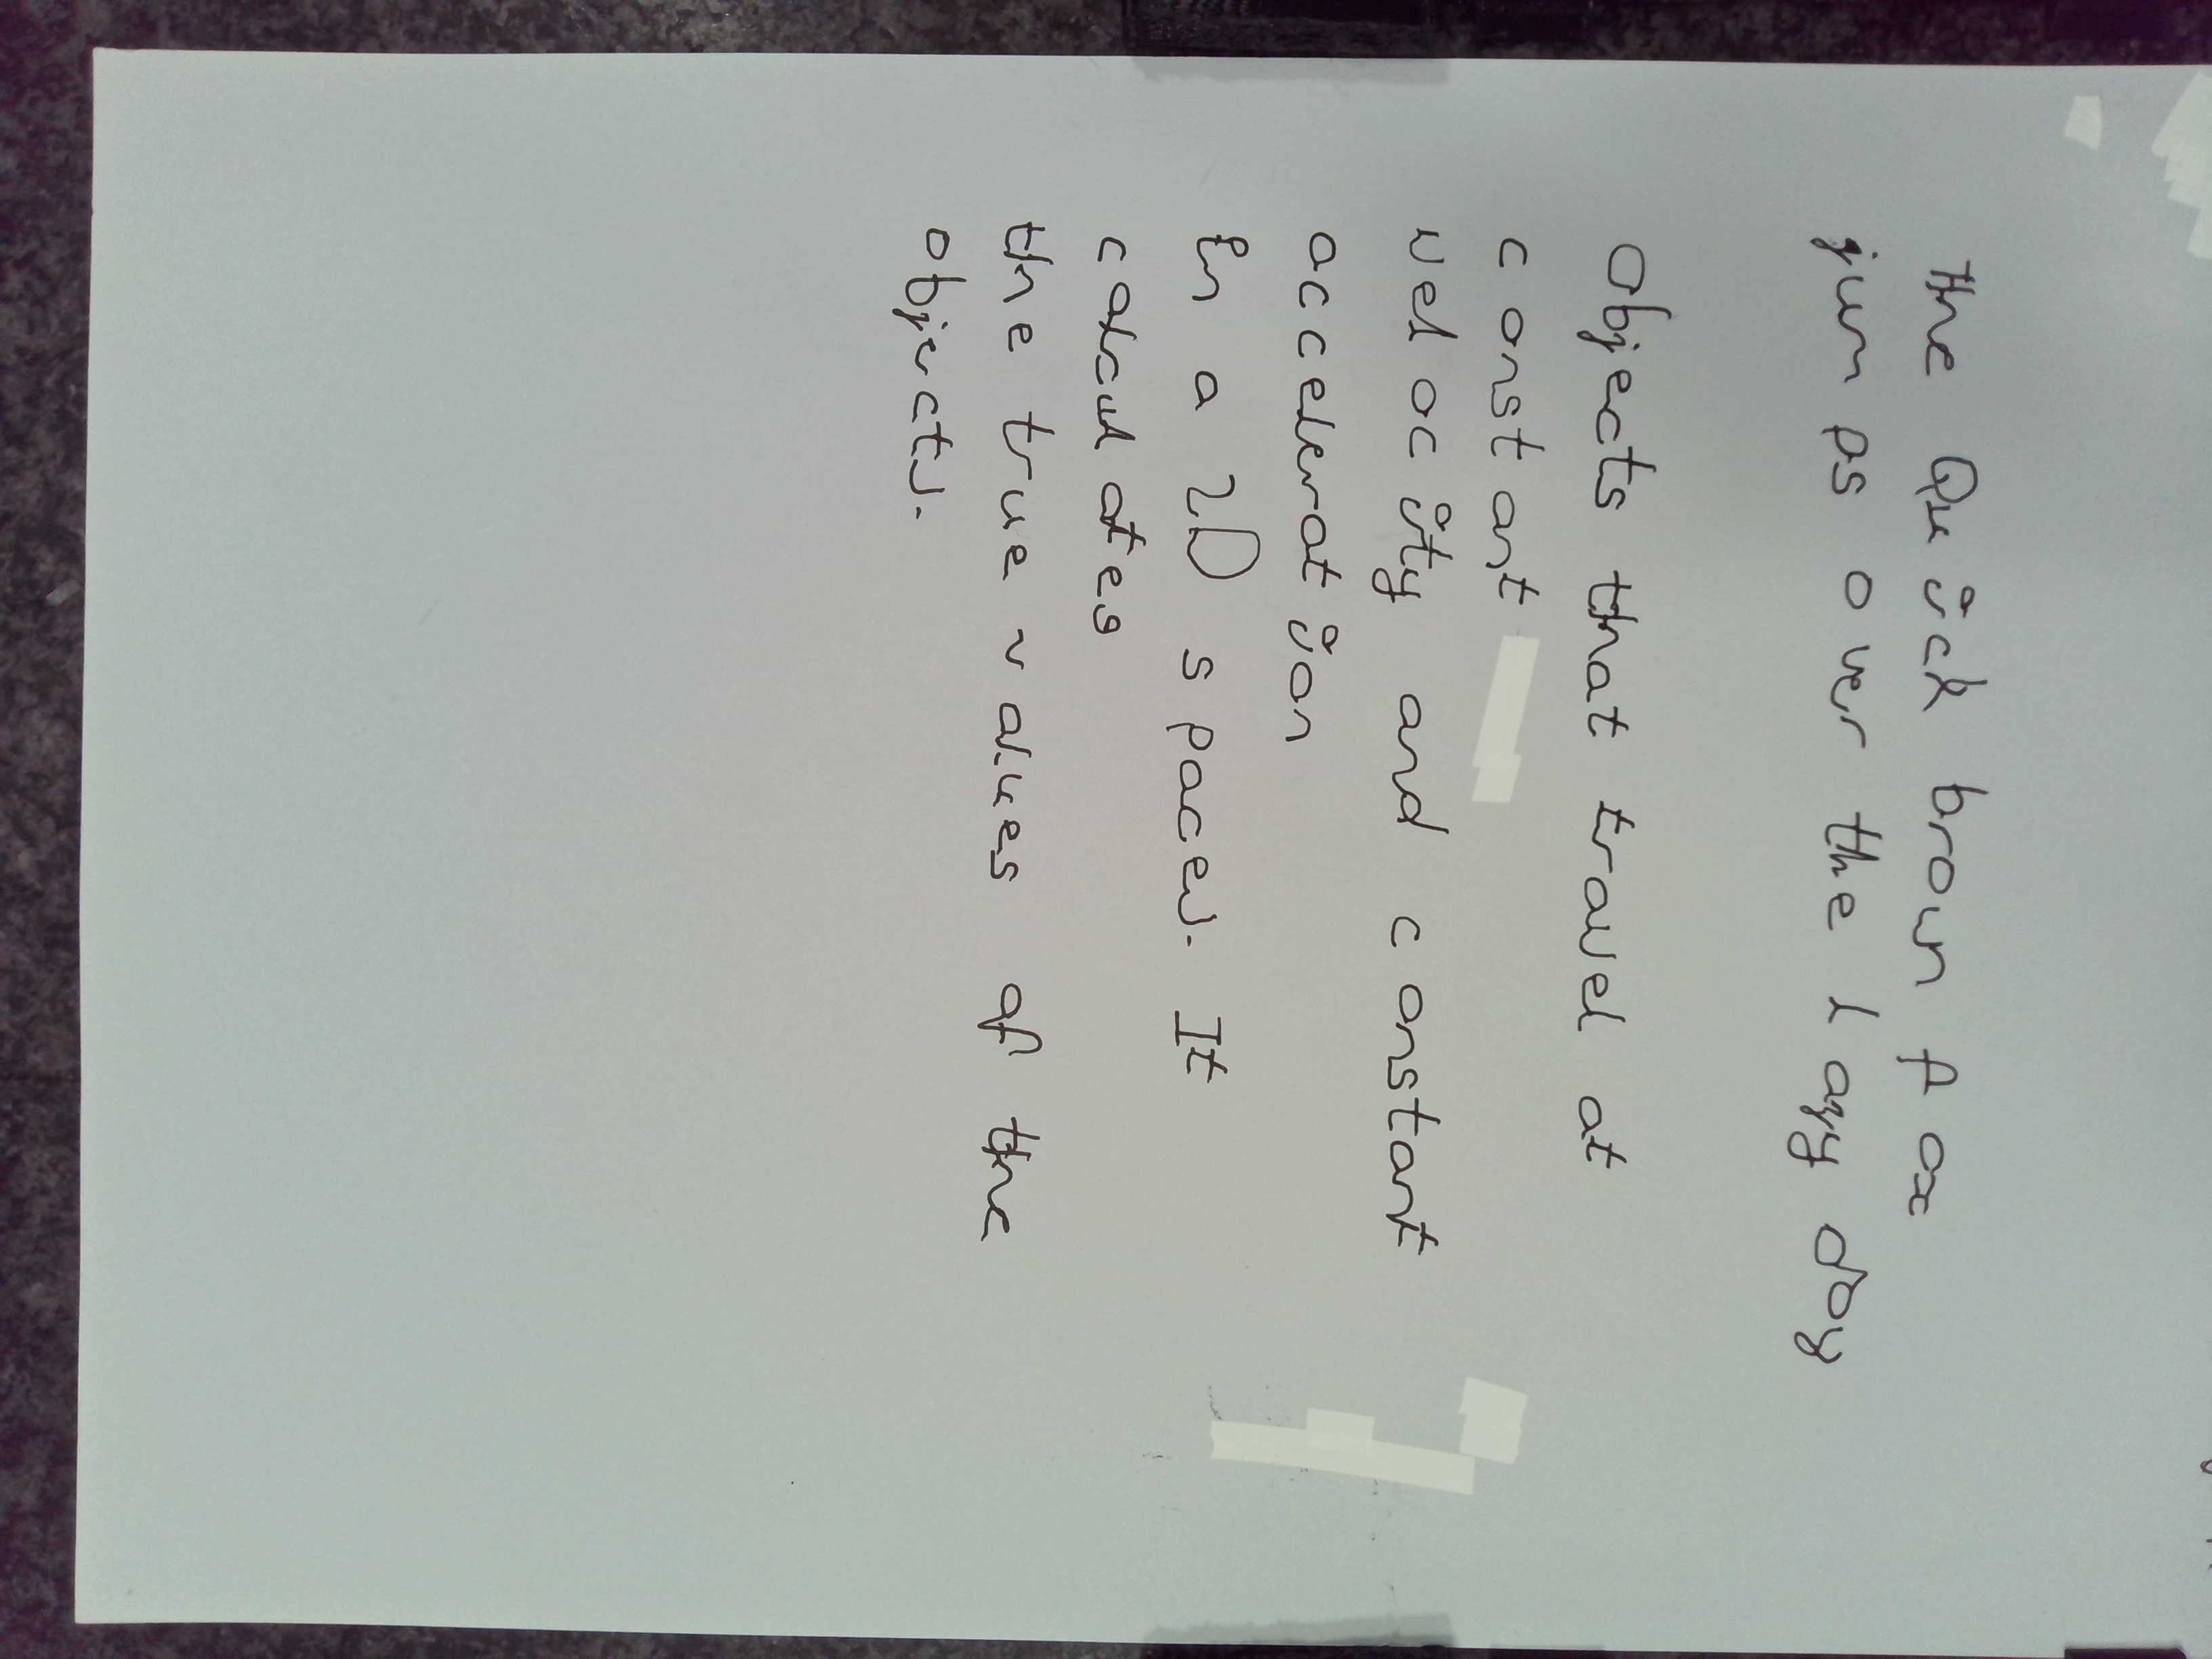
\includegraphics[angle=90,width=\linewidth,height=.55\textheight,keepaspectratio]{Figures/PhysicalPages/AuthorA2.jpg}\par AuthorA2\end{minipage}\hfill
\caption{Physical pages AuthorA1, AuthorA2.}\label{fig:app-physical-pages-5}\end{figure}\FloatBarrier

Figure~\ref{fig:app-physical-pages-6} preserves the photographed pages AuthorD, AuthorO. The scores come from their paired line records, not a visual estimate.
\begin{figure}[!htbp]\centering
\begin{minipage}{.48\linewidth}\centering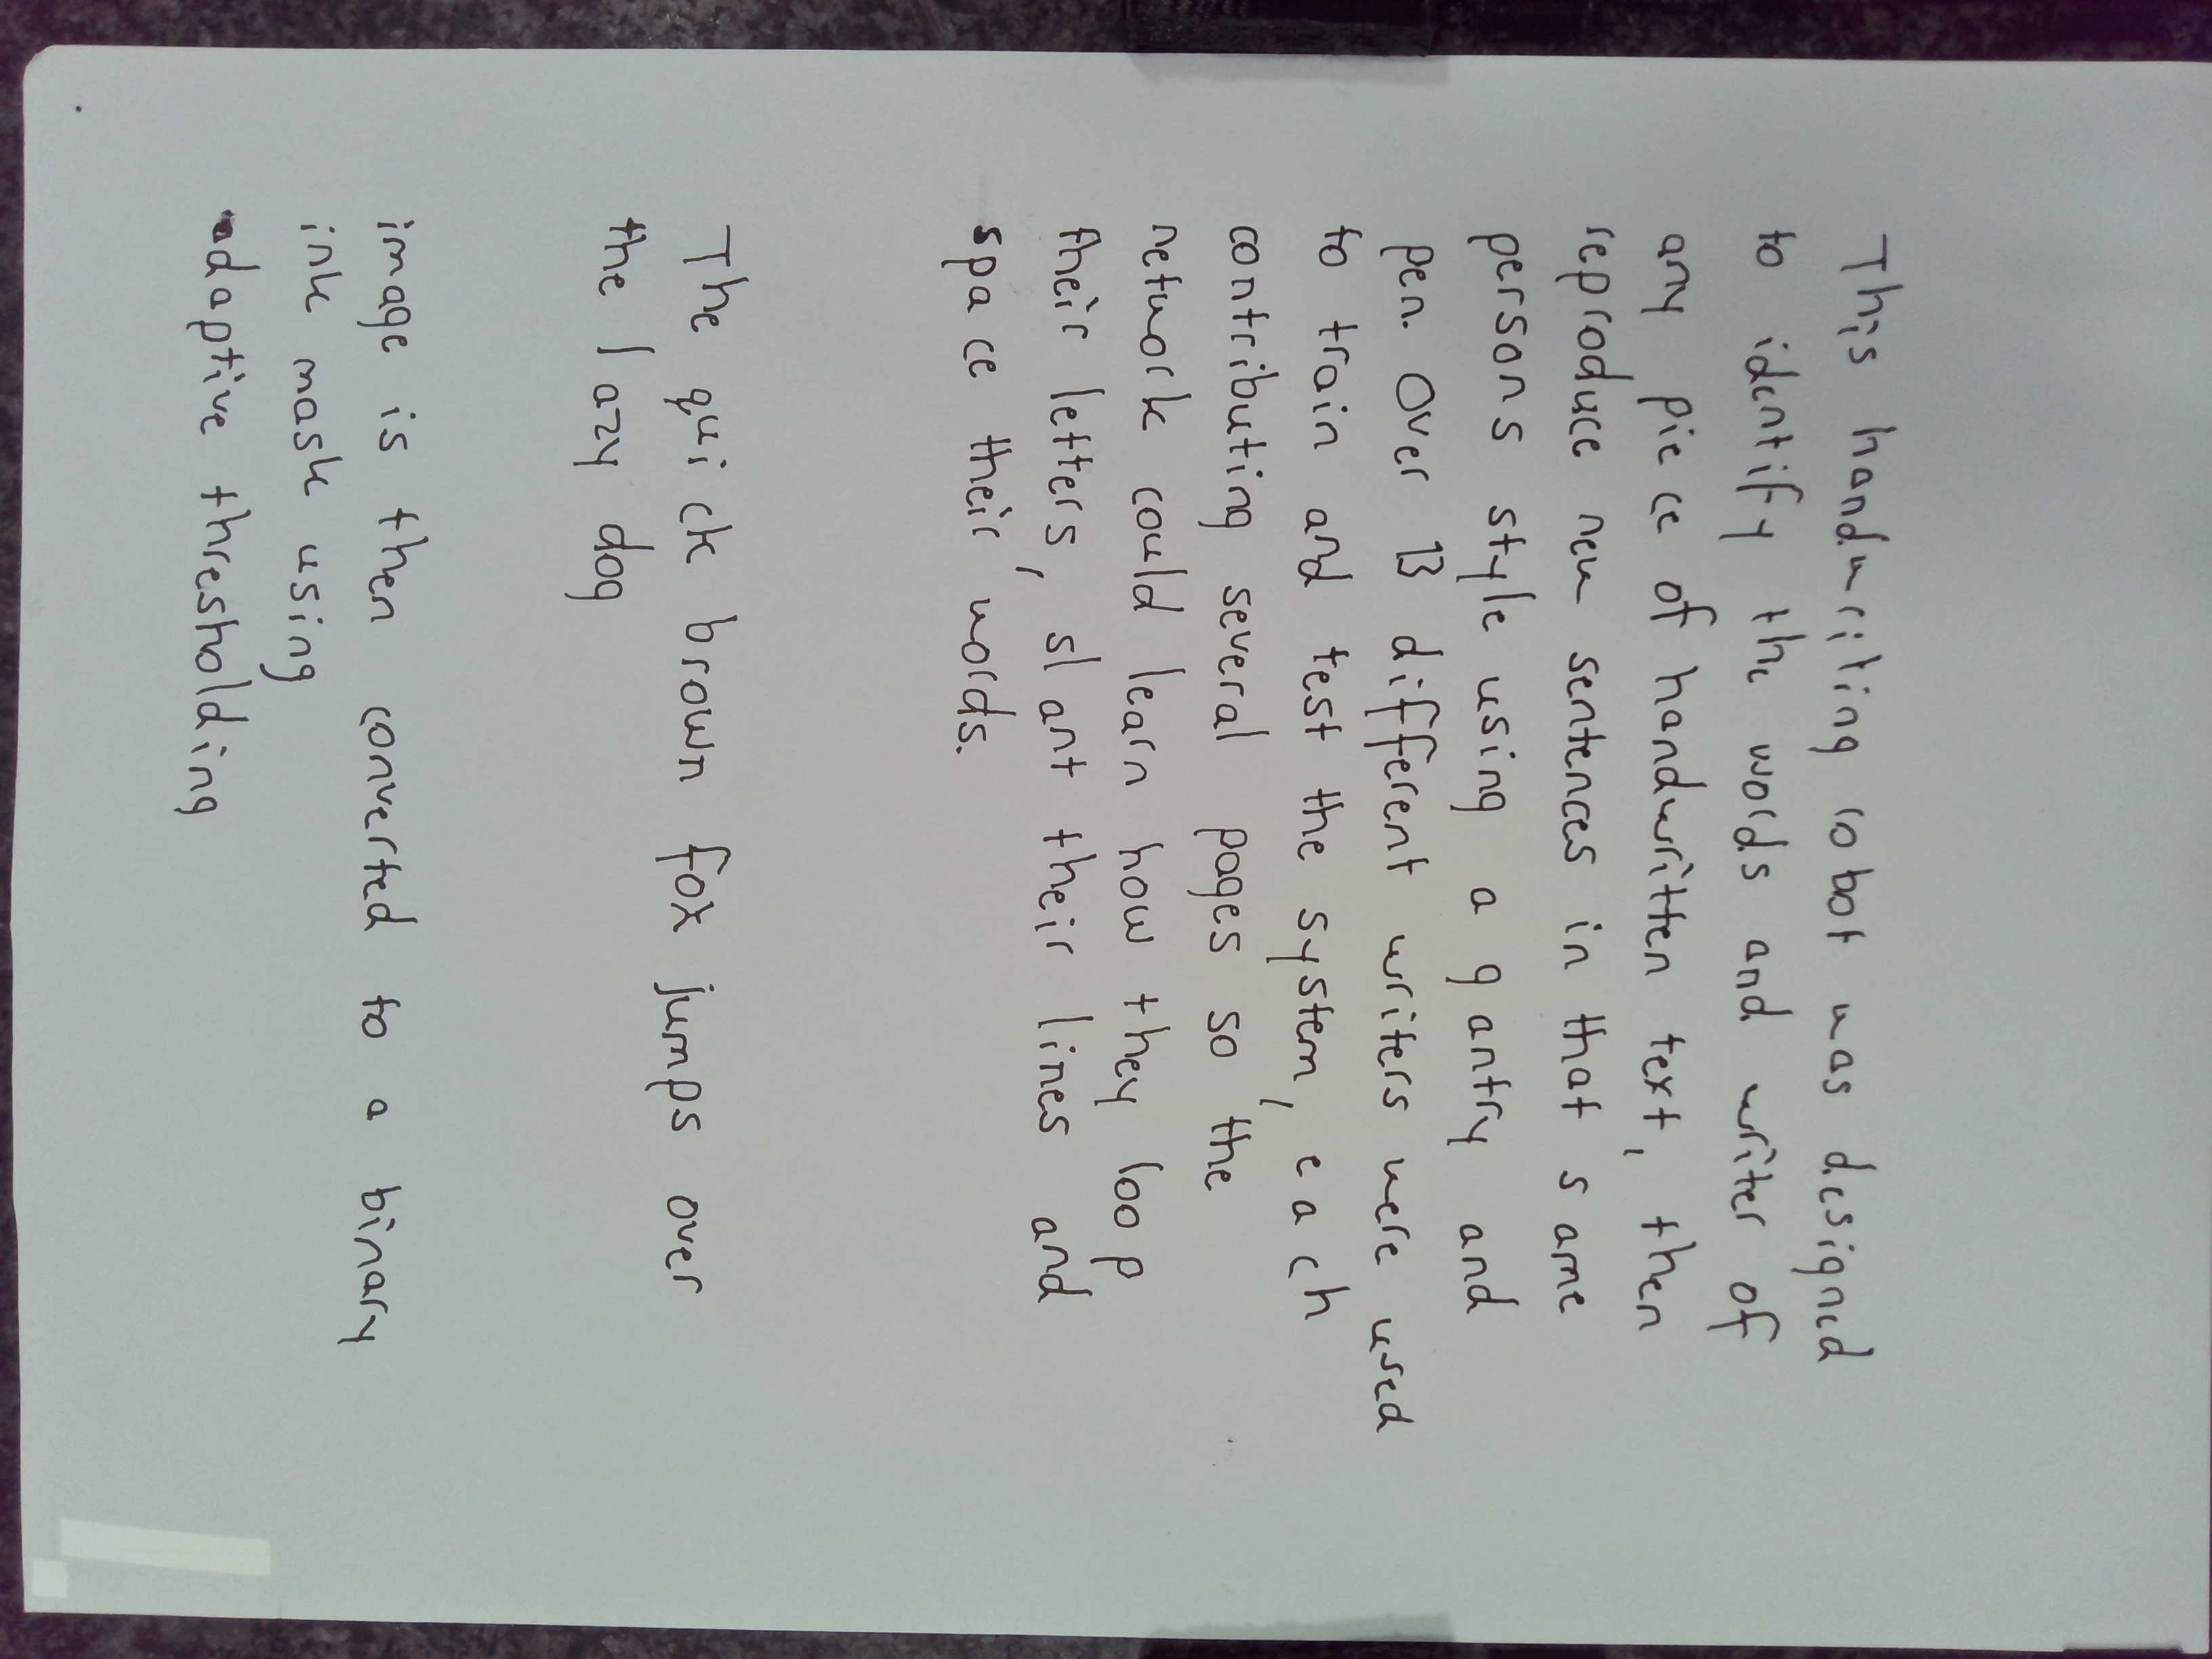
\includegraphics[angle=90,width=\linewidth,height=.55\textheight,keepaspectratio]{Figures/PhysicalPages/AuthorD.jpg}\par AuthorD\end{minipage}\hfill
\begin{minipage}{.48\linewidth}\centering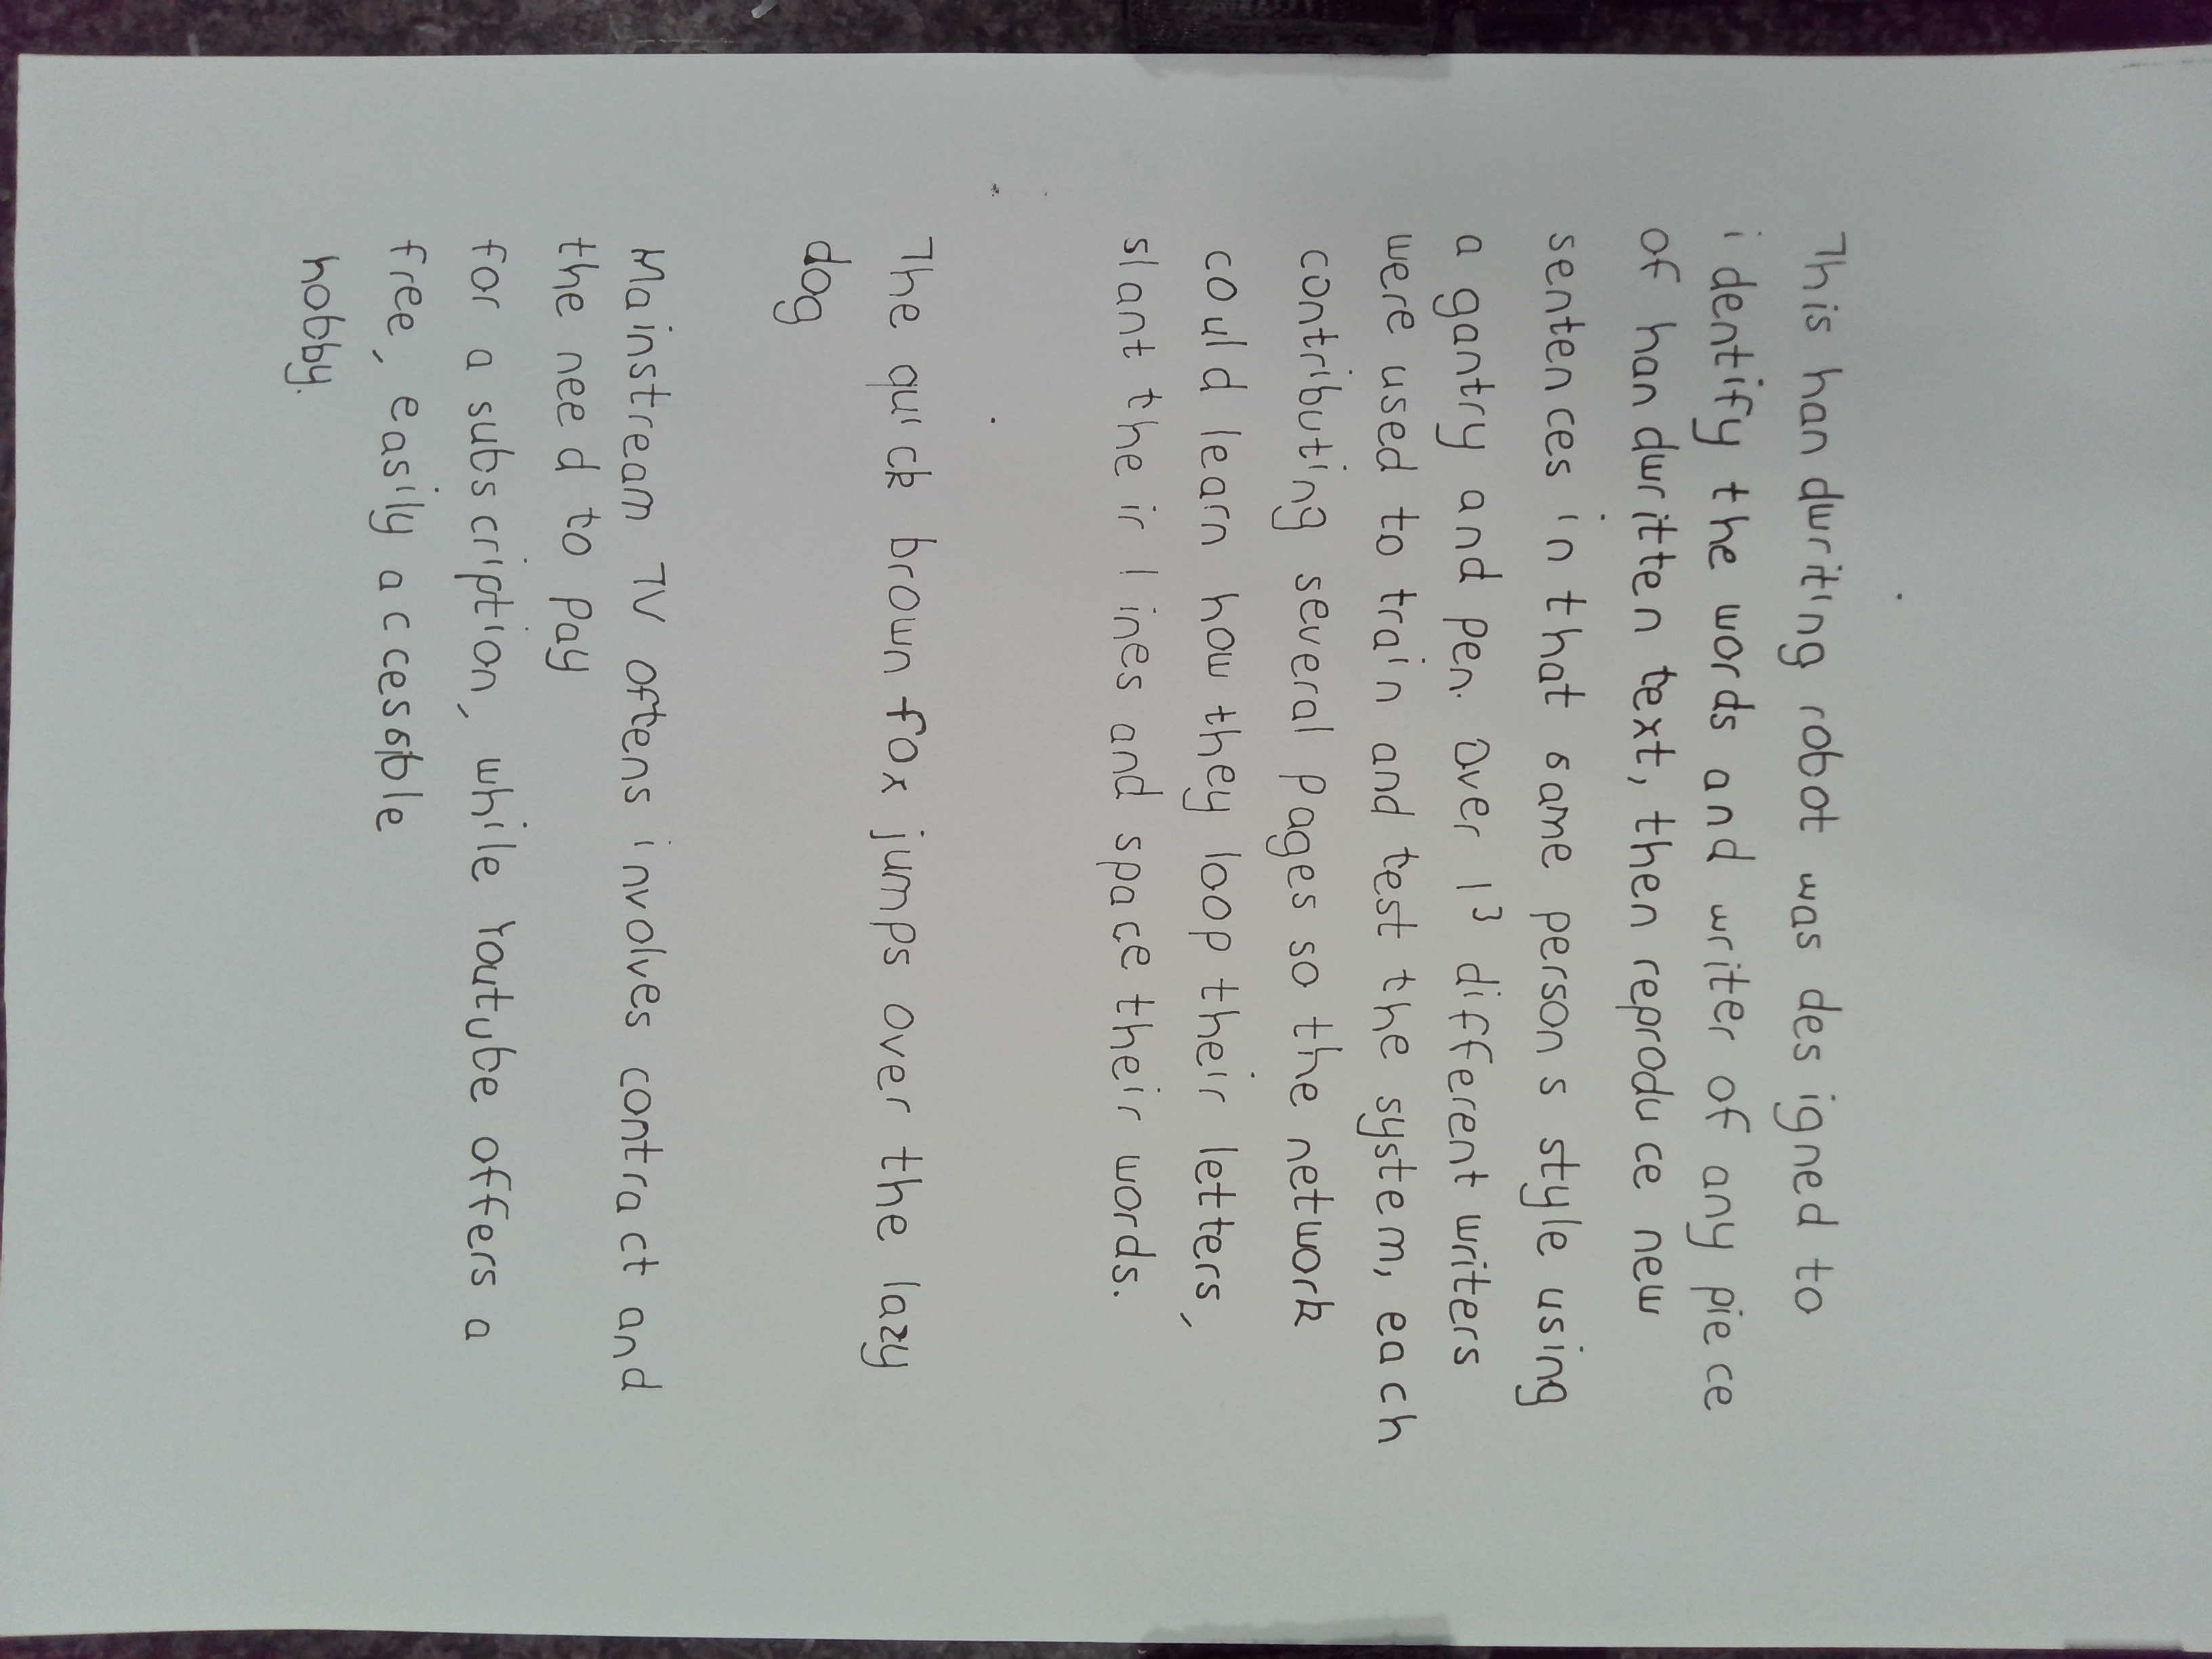
\includegraphics[angle=90,width=\linewidth,height=.55\textheight,keepaspectratio]{Figures/PhysicalPages/AuthorO.jpg}\par AuthorO\end{minipage}\hfill
\caption{Physical pages AuthorD, AuthorO.}\label{fig:app-physical-pages-6}\end{figure}\FloatBarrier

Figure~\ref{fig:app-physical-pages-7} preserves the photographed pages AuthorT, AuthorY. The scores come from their paired line records, not a visual estimate.
\begin{figure}[!htbp]\centering
\begin{minipage}{.48\linewidth}\centering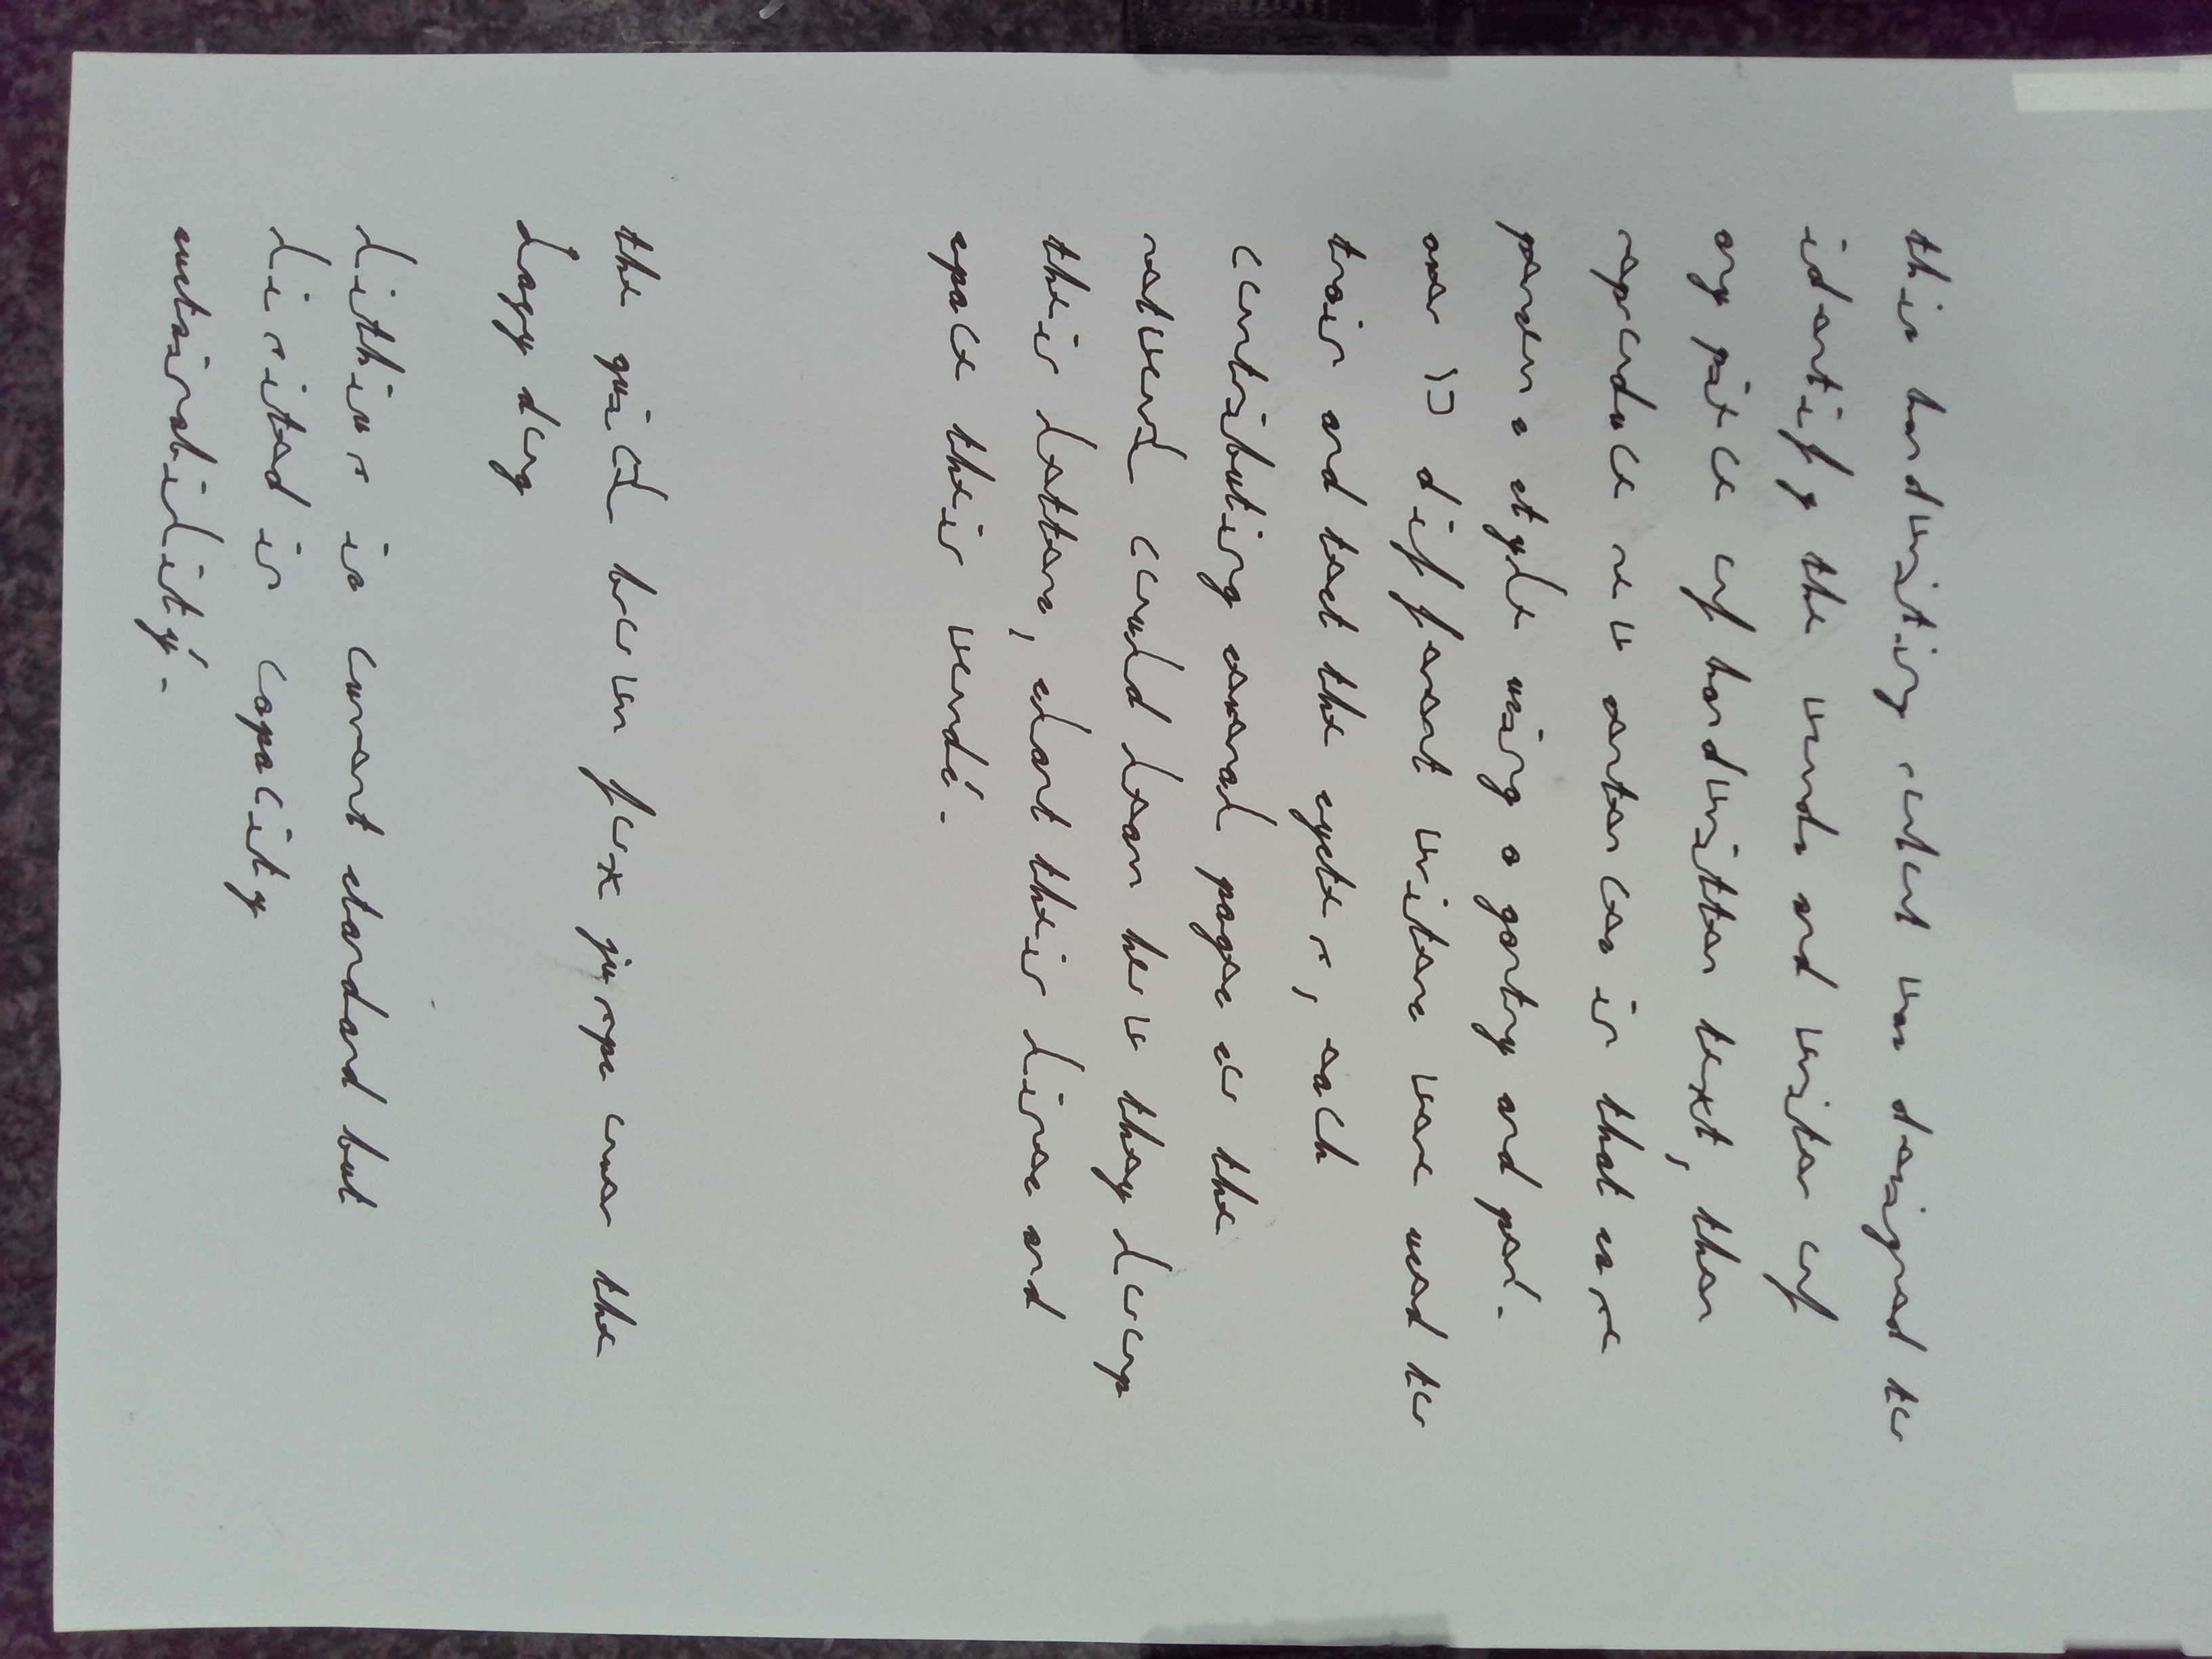
\includegraphics[angle=90,width=\linewidth,height=.55\textheight,keepaspectratio]{Figures/PhysicalPages/AuthorT.jpg}\par AuthorT\end{minipage}\hfill
\begin{minipage}{.48\linewidth}\centering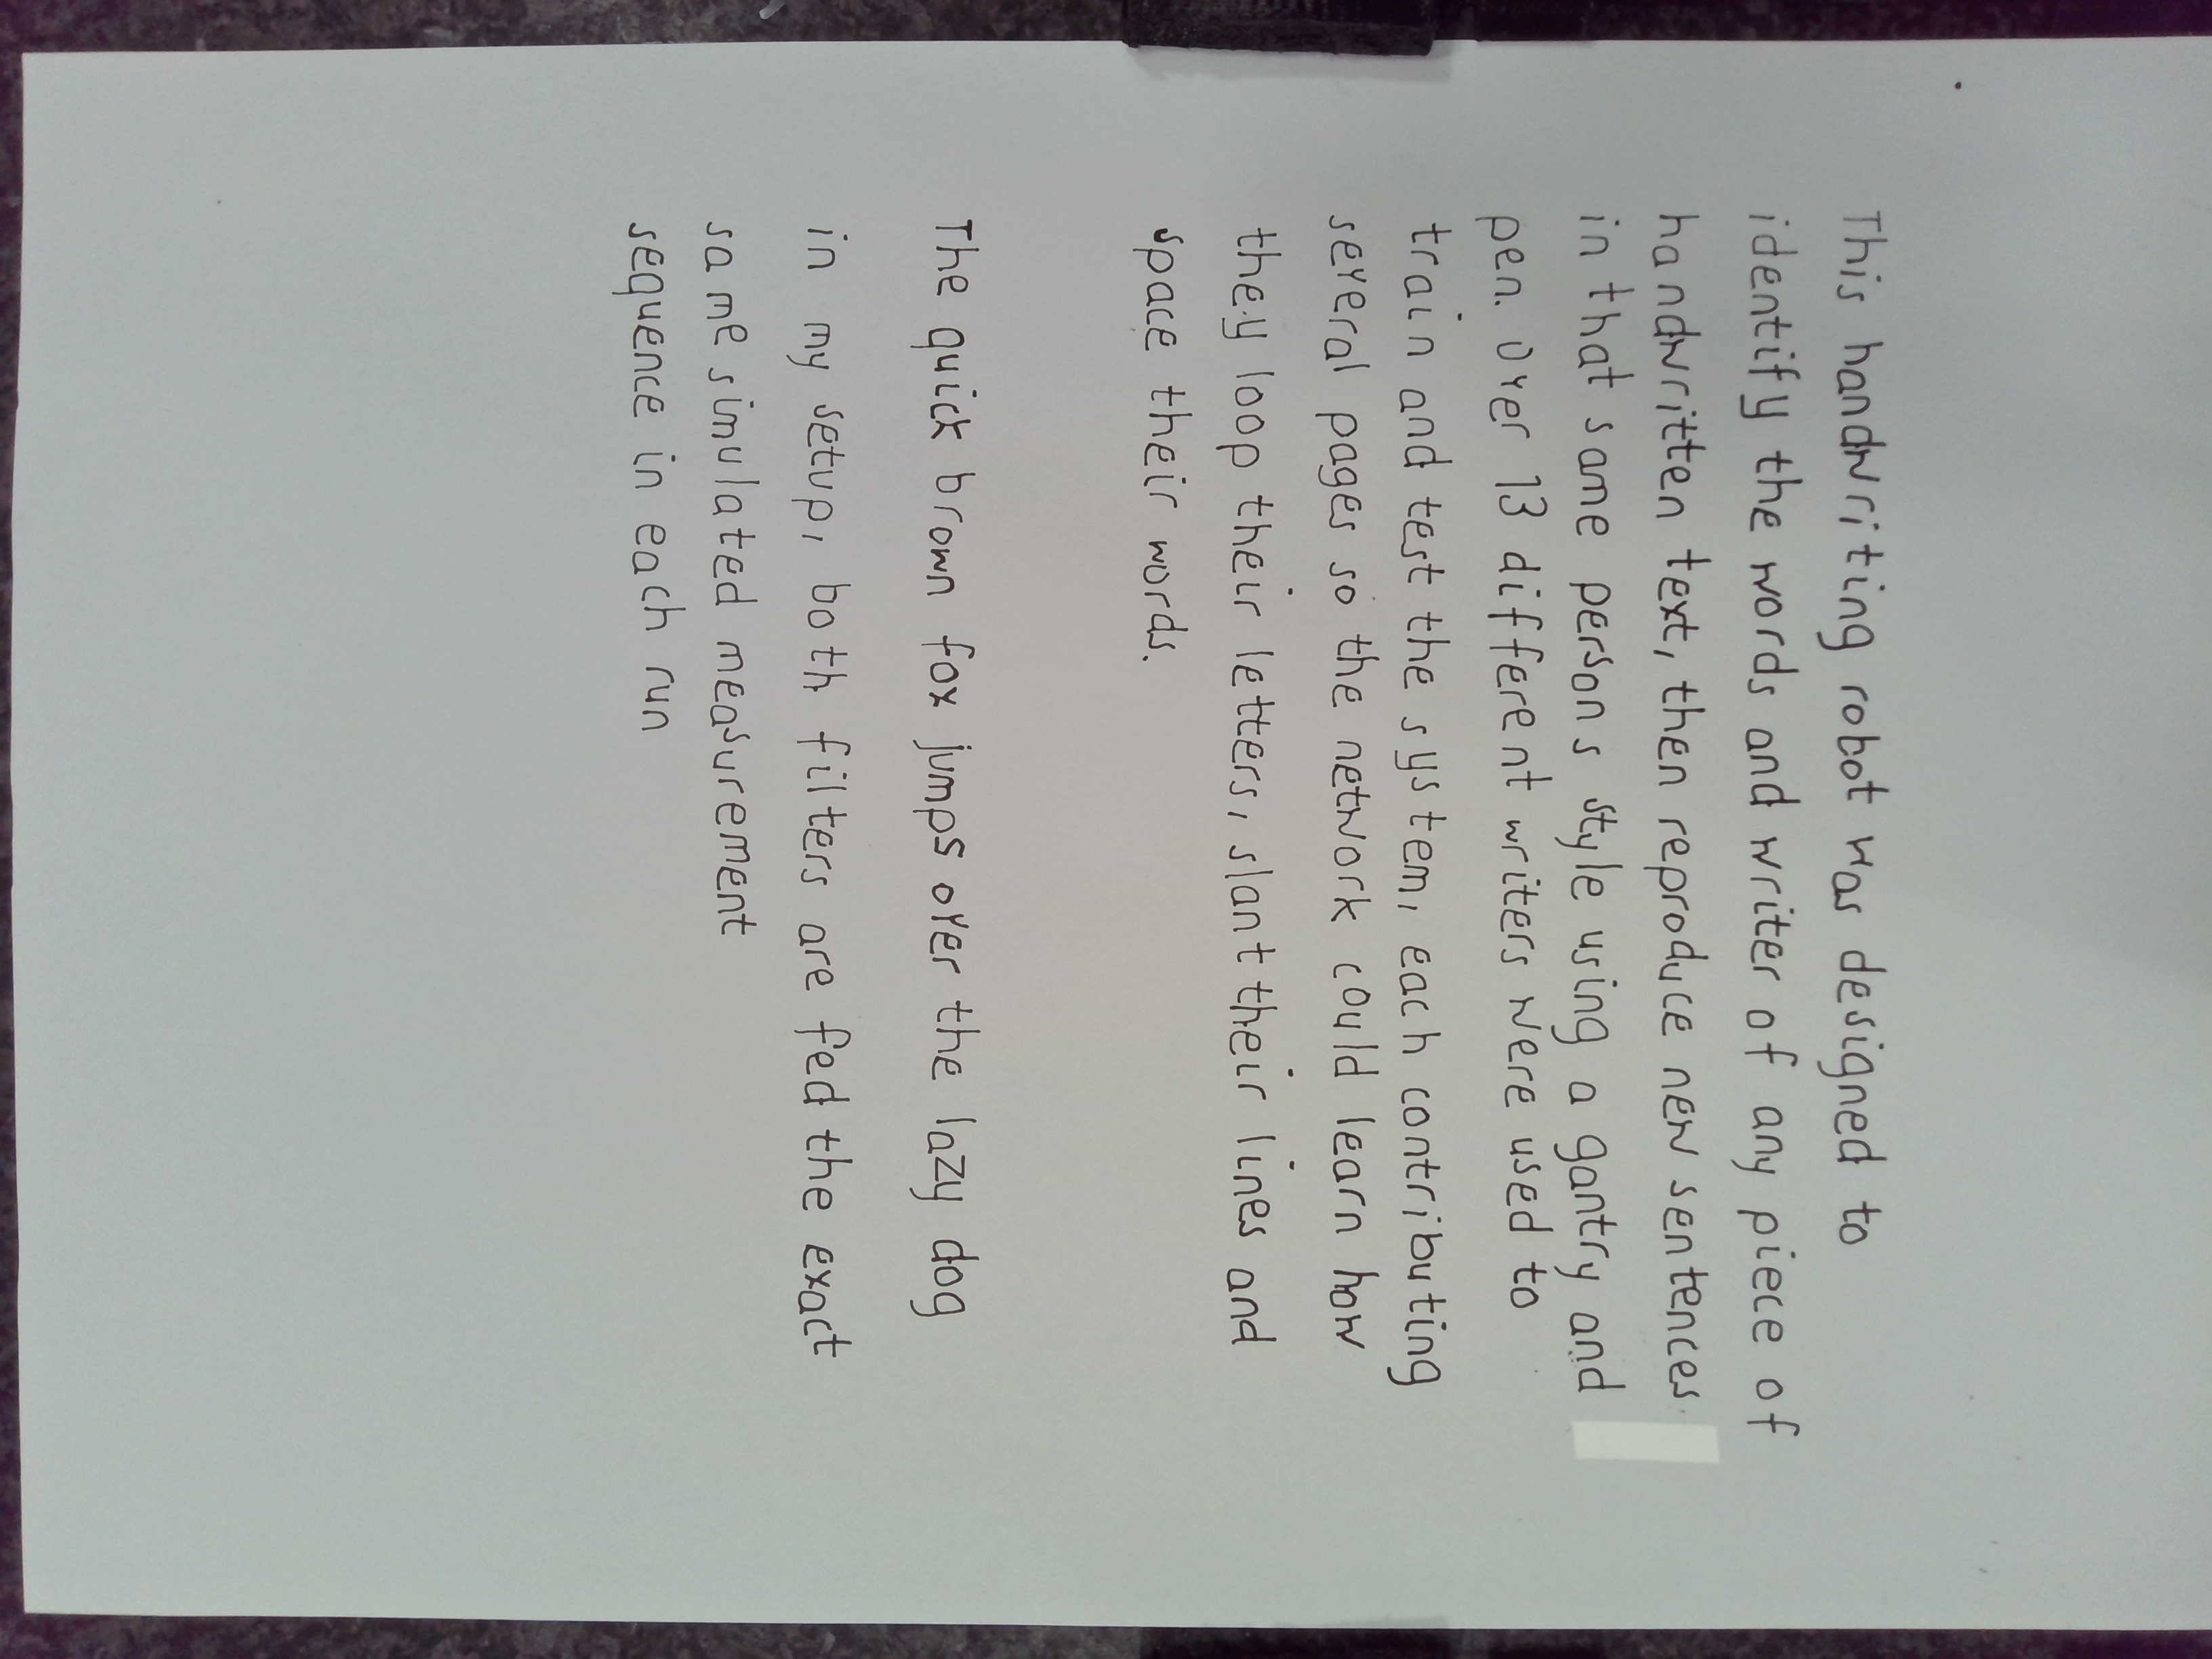
\includegraphics[angle=90,width=\linewidth,height=.55\textheight,keepaspectratio]{Figures/PhysicalPages/AuthorY.jpg}\par AuthorY\end{minipage}\hfill
\caption{Physical pages AuthorT, AuthorY.}\label{fig:app-physical-pages-7}\end{figure}\FloatBarrier

\subsection{Paired-line scoring record}
Table~\ref{tab:app-all-lines} gives every paired line, its reference length, edit distance and writer decision. Line numbering starts at one for each page. Reference and recognised text are retained verbatim in the accompanying evidence CSV so that these summaries can be recalculated.
\begin{longtable}{lrrrrl}
\caption{All 184 paired physical lines.}\label{tab:app-all-lines}\\
\toprule Page & Line & Characters & Edits & Character / \% & Predicted writer\\\midrule\endfirsthead
\toprule Page & Line & Characters & Edits & Character / \% & Predicted writer\\\midrule\endhead
Author150 & 1 & 51 & 2 & 96.08 & 150\\
Author150 & 2 & 50 & 1 & 98.00 & Y\\
Author150 & 3 & 50 & 1 & 98.00 & 150\\
Author150 & 4 & 47 & 3 & 93.62 & Y\\
Author150 & 5 & 52 & 1 & 98.08 & Y\\
Author150 & 6 & 47 & 3 & 93.62 & 150\\
Author150 & 7 & 52 & 1 & 98.08 & Y\\
Author150 & 8 & 22 & 0 & 100.00 & 150\\
Author150 & 9 & 39 & 2 & 94.87 & 150\\
Author150 & 10 & 3 & 1 & 66.67 & O\\
Author150 & 11 & 38 & 1 & 97.37 & 150\\
Author150 & 12 & 36 & 0 & 100.00 & 150\\
Author150 & 13 & 6 & 0 & 100.00 & Y\\
Author152 & 1 & 38 & 4 & 89.47 & 152\\
Author152 & 2 & 36 & 5 & 86.11 & 152\\
Author152 & 3 & 41 & 4 & 90.24 & 152\\
Author152 & 4 & 41 & 7 & 82.93 & 588\\
Author152 & 5 & 31 & 1 & 96.77 & 152\\
Author152 & 6 & 40 & 6 & 85.00 & 152\\
Author152 & 7 & 42 & 6 & 85.71 & 152\\
Author152 & 8 & 36 & 3 & 91.67 & 152\\
Author152 & 9 & 42 & 6 & 85.71 & 152\\
Author152 & 10 & 22 & 3 & 86.36 & 152\\
Author152 & 11 & 34 & 7 & 79.41 & 152\\
Author152 & 12 & 8 & 3 & 62.50 & Y\\
Author152 & 13 & 33 & 7 & 78.79 & 152\\
Author152 & 14 & 37 & 5 & 86.49 & 152\\
Author152 & 15 & 10 & 3 & 70.00 & T\\
Author1531 & 1 & 26 & 12 & 53.85 & 153\\
Author1531 & 2 & 30 & 8 & 73.33 & 153\\
Author1531 & 3 & 26 & 4 & 84.62 & 153\\
Author1531 & 4 & 32 & 6 & 81.25 & 153\\
Author1531 & 5 & 26 & 4 & 84.62 & 384\\
Author1531 & 6 & 28 & 6 & 78.57 & T\\
Author1531 & 7 & 26 & 8 & 69.23 & T\\
Author1531 & 8 & 30 & 7 & 76.67 & 588\\
Author1531 & 9 & 21 & 5 & 76.19 & 153\\
Author1531 & 10 & 33 & 10 & 69.70 & 153\\
Author1531 & 11 & 28 & 8 & 71.43 & 153\\
Author1531 & 12 & 31 & 7 & 77.42 & T\\
Author1531 & 13 & 28 & 8 & 71.43 & 153\\
Author1531 & 14 & 30 & 10 & 66.67 & 153\\
Author1531 & 15 & 12 & 3 & 75.00 & T\\
Author1532 & 1 & 29 & 5 & 82.76 & 153\\
Author1532 & 2 & 29 & 3 & 89.66 & 153\\
Author1532 & 3 & 11 & 4 & 63.64 & T\\
Author1532 & 4 & 10 & 0 & 100.00 & T\\
Author3841 & 1 & 35 & 2 & 94.29 & 384\\
Author3841 & 2 & 35 & 2 & 94.29 & 384\\
Author3841 & 3 & 35 & 7 & 80.00 & 384\\
Author3841 & 4 & 36 & 3 & 91.67 & 384\\
Author3841 & 5 & 32 & 2 & 93.75 & 384\\
Author3841 & 6 & 35 & 3 & 91.43 & 384\\
Author3841 & 7 & 34 & 4 & 88.24 & 384\\
Author3841 & 8 & 34 & 6 & 82.35 & 384\\
Author3841 & 9 & 32 & 5 & 84.38 & 384\\
Author3841 & 10 & 31 & 4 & 87.10 & 384\\
Author3841 & 11 & 28 & 4 & 85.71 & 384\\
Author3841 & 12 & 34 & 7 & 79.41 & 384\\
Author3841 & 13 & 8 & 3 & 62.50 & A\\
Author3842 & 1 & 34 & 6 & 82.35 & 384\\
Author3842 & 2 & 10 & 1 & 90.00 & O\\
Author3842 & 3 & 29 & 4 & 86.21 & 384\\
Author552 & 1 & 38 & 6 & 84.21 & 552\\
Author552 & 2 & 45 & 5 & 88.89 & 552\\
Author552 & 3 & 36 & 4 & 88.89 & 552\\
Author552 & 4 & 44 & 2 & 95.45 & 552\\
Author552 & 5 & 46 & 12 & 73.91 & 552\\
Author552 & 6 & 39 & 1 & 97.44 & 552\\
Author552 & 7 & 47 & 4 & 91.49 & 552\\
Author552 & 8 & 46 & 5 & 89.13 & 552\\
Author552 & 9 & 28 & 3 & 89.29 & 552\\
Author552 & 10 & 34 & 6 & 82.35 & 552\\
Author552 & 11 & 8 & 2 & 75.00 & A\\
Author552 & 12 & 34 & 5 & 85.29 & 552\\
Author552 & 13 & 14 & 4 & 71.43 & A\\
Author552 & 14 & 16 & 4 & 75.00 & A\\
Author552 & 15 & 31 & 7 & 77.42 & 552\\
Author588 & 1 & 34 & 5 & 85.29 & 588\\
Author588 & 2 & 8 & 2 & 75.00 & 588\\
Author588 & 3 & 32 & 8 & 75.00 & 588\\
Author588 & 4 & 10 & 4 & 60.00 & 588\\
Author588 & 5 & 27 & 4 & 85.19 & 588\\
Author588 & 6 & 13 & 7 & 46.15 & 588\\
Author588 & 7 & 5 & 4 & 20.00 & A\\
Author588 & 8 & 35 & 10 & 71.43 & 588\\
Author588 & 9 & 35 & 7 & 80.00 & 588\\
Author588 & 10 & 35 & 13 & 62.86 & 588\\
Author588 & 11 & 36 & 13 & 63.89 & 588\\
Author588 & 12 & 37 & 6 & 83.78 & 588\\
Author588 & 13 & 38 & 6 & 84.21 & 588\\
Author588 & 14 & 31 & 11 & 64.52 & 588\\
Author588 & 15 & 33 & 10 & 69.70 & 588\\
Author588 & 16 & 33 & 11 & 66.67 & 588\\
Author588 & 17 & 36 & 5 & 86.11 & 588\\
Author588 & 18 & 18 & 7 & 61.11 & 588\\
AuthorA1 & 1 & 22 & 12 & 45.45 & A\\
AuthorA1 & 2 & 24 & 7 & 70.83 & A\\
AuthorA1 & 3 & 23 & 4 & 82.61 & A\\
AuthorA1 & 4 & 12 & 2 & 83.33 & A\\
AuthorA1 & 5 & 22 & 5 & 77.27 & A\\
AuthorA1 & 6 & 23 & 1 & 95.65 & A\\
AuthorA1 & 7 & 20 & 4 & 80.00 & A\\
AuthorA1 & 8 & 24 & 3 & 87.50 & A\\
AuthorA1 & 9 & 22 & 5 & 77.27 & A\\
AuthorA1 & 10 & 20 & 5 & 75.00 & A\\
AuthorA1 & 11 & 18 & 2 & 88.89 & A\\
AuthorA1 & 12 & 25 & 4 & 84.00 & A\\
AuthorA1 & 13 & 20 & 4 & 80.00 & A\\
AuthorA1 & 14 & 23 & 6 & 73.91 & A\\
AuthorA1 & 15 & 24 & 6 & 75.00 & A\\
AuthorA1 & 16 & 21 & 6 & 71.43 & A\\
AuthorA1 & 17 & 18 & 6 & 66.67 & A\\
AuthorA2 & 1 & 19 & 8 & 57.89 & A\\
AuthorA2 & 2 & 23 & 9 & 60.87 & A\\
AuthorA2 & 3 & 22 & 1 & 95.45 & A\\
AuthorA2 & 4 & 8 & 2 & 75.00 & A\\
AuthorA2 & 5 & 21 & 4 & 80.95 & A\\
AuthorA2 & 6 & 12 & 1 & 91.67 & A\\
AuthorA2 & 7 & 18 & 4 & 77.78 & A\\
AuthorA2 & 8 & 10 & 3 & 70.00 & A\\
AuthorA2 & 9 & 22 & 4 & 81.82 & A\\
AuthorA2 & 10 & 8 & 1 & 87.50 & A\\
AuthorD & 1 & 35 & 5 & 85.71 & B\\
AuthorD & 2 & 35 & 3 & 91.43 & B\\
AuthorD & 3 & 35 & 2 & 94.29 & B\\
AuthorD & 4 & 36 & 3 & 91.67 & B\\
AuthorD & 5 & 32 & 0 & 100.00 & B\\
AuthorD & 6 & 40 & 4 & 90.00 & B\\
AuthorD & 7 & 34 & 3 & 91.18 & B\\
AuthorD & 8 & 33 & 0 & 100.00 & B\\
AuthorD & 9 & 33 & 5 & 84.85 & B\\
AuthorD & 10 & 36 & 1 & 97.22 & B\\
AuthorD & 11 & 18 & 1 & 94.44 & B\\
AuthorD & 12 & 30 & 1 & 96.67 & B\\
AuthorD & 13 & 12 & 1 & 91.67 & B\\
AuthorD & 14 & 35 & 0 & 100.00 & B\\
AuthorD & 15 & 14 & 2 & 85.71 & 552\\
AuthorD & 16 & 21 & 2 & 90.48 & B\\
AuthorO & 1 & 38 & 3 & 92.11 & O\\
AuthorO & 2 & 42 & 2 & 95.24 & O\\
AuthorO & 3 & 39 & 2 & 94.87 & O\\
AuthorO & 4 & 42 & 0 & 100.00 & O\\
AuthorO & 5 & 43 & 3 & 93.02 & O\\
AuthorO & 6 & 44 & 2 & 95.45 & O\\
AuthorO & 7 & 41 & 1 & 97.56 & O\\
AuthorO & 8 & 40 & 1 & 97.50 & O\\
AuthorO & 9 & 40 & 2 & 95.00 & O\\
AuthorO & 10 & 39 & 4 & 89.74 & O\\
AuthorO & 11 & 3 & 1 & 66.67 & O\\
AuthorO & 12 & 42 & 1 & 97.62 & O\\
AuthorO & 13 & 15 & 2 & 86.67 & O\\
AuthorO & 14 & 42 & 3 & 92.86 & O\\
AuthorO & 15 & 23 & 3 & 86.96 & O\\
AuthorO & 16 & 6 & 1 & 83.33 & O\\
AuthorT & 1 & 38 & 16 & 57.89 & T\\
AuthorT & 2 & 32 & 8 & 75.00 & T\\
AuthorT & 3 & 35 & 13 & 62.86 & T\\
AuthorT & 4 & 36 & 15 & 58.33 & T\\
AuthorT & 5 & 37 & 12 & 67.57 & T\\
AuthorT & 6 & 38 & 16 & 57.89 & T\\
AuthorT & 7 & 31 & 9 & 70.97 & T\\
AuthorT & 8 & 33 & 12 & 63.64 & T\\
AuthorT & 9 & 33 & 22 & 33.33 & T\\
AuthorT & 10 & 36 & 12 & 66.67 & T\\
AuthorT & 11 & 18 & 6 & 66.67 & T\\
AuthorT & 12 & 34 & 20 & 41.18 & T\\
AuthorT & 13 & 8 & 5 & 37.50 & T\\
AuthorT & 14 & 31 & 10 & 67.74 & T\\
AuthorT & 15 & 19 & 4 & 78.95 & T\\
AuthorT & 16 & 15 & 5 & 66.67 & T\\
AuthorY & 1 & 38 & 2 & 94.74 & Y\\
AuthorY & 2 & 45 & 1 & 97.78 & Y\\
AuthorY & 3 & 46 & 0 & 100.00 & Y\\
AuthorY & 4 & 45 & 2 & 95.56 & Y\\
AuthorY & 5 & 43 & 4 & 90.70 & Y\\
AuthorY & 6 & 44 & 2 & 95.45 & Y\\
AuthorY & 7 & 44 & 1 & 97.73 & Y\\
AuthorY & 8 & 46 & 0 & 100.00 & Y\\
AuthorY & 9 & 18 & 0 & 100.00 & Y\\
AuthorY & 10 & 43 & 0 & 100.00 & Y\\
AuthorY & 11 & 43 & 1 & 97.67 & Y\\
AuthorY & 12 & 26 & 2 & 92.31 & Y\\
AuthorY & 13 & 20 & 0 & 100.00 & O\\
\bottomrule\end{longtable}

\subsection{Complete confirmed reproduction timings}
Table~\ref{tab:app-complete-timings} retains the 25 completed, positive-character records used in QT~3. The line number identifies the timing block in the preserved ODROID log. Synthesis and drawing are component stages. The total also includes the other logged stages and rounding, so it is not replaced by their sum.
\begin{longtable}{rrrrrr}
\caption{All confirmed ODROID reproduction timings.}\label{tab:app-complete-timings}\\
\toprule Log line & Characters & Synthesis / s & Drawing / s & Total / s & s per character\\\midrule\endfirsthead
\toprule Log line & Characters & Synthesis / s & Drawing / s & Total / s & s per character\\\midrule\endhead
32 & 378 & 8.23 & 497.55 & 507.57 & 1.343\\
185 & 378 & 17.98 & 637.31 & 657.72 & 1.740\\
203 & 43 & 17.66 & 92.59 & 110.59 & 2.572\\
595 & 91 & 16.44 & 175.50 & 192.47 & 2.115\\
631 & 378 & 12.36 & 651.18 & 665.14 & 1.760\\
682 & 43 & 14.80 & 91.30 & 106.44 & 2.475\\
718 & 82 & 17.06 & 165.46 & 183.04 & 2.232\\
816 & 378 & 39.27 & 899.55 & 941.48 & 2.491\\
864 & 43 & 20.34 & 113.94 & 134.65 & 3.131\\
887 & 82 & 27.53 & 204.05 & 232.16 & 2.831\\
1004 & 378 & 58.78 & 1022.83 & 1085.01 & 2.870\\
1027 & 43 & 26.52 & 139.66 & 166.61 & 3.875\\
1050 & 82 & 33.67 & 225.88 & 260.33 & 3.175\\
1099 & 378 & 16.63 & 839.33 & 859.00 & 2.272\\
1122 & 43 & 18.81 & 106.99 & 126.19 & 2.935\\
1145 & 75 & 25.39 & 162.76 & 188.60 & 2.515\\
1189 & 378 & 12.11 & 663.01 & 676.64 & 1.790\\
1225 & 43 & 15.10 & 96.53 & 112.00 & 2.605\\
1260 & 43 & 15.22 & 96.44 & 112.03 & 2.605\\
1348 & 378 & 104.08 & 656.92 & 762.84 & 2.018\\
1384 & 43 & 15.65 & 81.40 & 97.28 & 2.262\\
1407 & 91 & 23.34 & 198.59 & 222.63 & 2.446\\
1495 & 378 & 14.17 & 726.40 & 742.72 & 1.965\\
1518 & 43 & 15.19 & 95.64 & 111.18 & 2.586\\
1541 & 132 & 22.88 & 254.16 & 277.90 & 2.105\\
\bottomrule\end{longtable}


\subsection{Supplied first-principles training records}\label{app:training-records}
The following tables transcribe the console excerpts supplied by the author. They extend the training-route comparison in Design. The writer run uses 1031 training and 155 validation lines, eleven writers and 0.17 stroke width. Its output is \texttt{author\_shape\_11w\_pw170\_scratch\_weights.npz}. Table~\ref{tab:app-author-log} retains the displayed values. The excerpt ends with an interruption after epoch 47, rather than a completed 50-epoch run.
\begin{longtable}{rrrr}
\caption{Supplied numerical writer training log.}\label{tab:app-author-log}\\
\toprule Epoch & Loss & Validation / \% & Time / min\\\midrule\endfirsthead
\toprule Epoch & Loss & Validation / \% & Time / min\\\midrule\endhead
1 & 1.979 & 47.7 & 20.1\\
2 & 1.393 & 54.2 & 19.7\\
3 & 1.178 & 58.1 & 19.9\\
4 & 0.985 & 34.2 & 21.6\\
5 & 0.817 & 72.3 & 22.1\\
6 & 0.726 & 59.4 & 22.7\\
7 & 0.730 & 43.9 & 22.1\\
8 & 0.642 & 59.4 & 21.7\\
9 & 0.578 & 73.5 & 20.3\\
10 & 0.531 & 87.7 & 20.1\\
11 & 0.532 & 66.5 & 20.8\\
12 & 0.499 & 80.6 & 20.4\\
13 & 0.465 & 63.9 & 20.6\\
14 & 0.404 & 89.7 & 20.6\\
15 & 0.442 & 59.4 & 20.7\\
16 & 0.373 & 63.2 & 20.1\\
17 & 0.313 & 84.5 & 20.2\\
18 & 0.378 & 94.2 & 20.6\\
19 & 0.265 & 86.5 & 19.4\\
20 & 0.344 & 86.5 & 19.5\\
21 & 0.294 & 90.3 & 19.8\\
22 & 0.319 & 92.3 & 19.7\\
23 & 0.250 & 89.0 & 19.4\\
24 & 0.233 & 93.5 & 19.4\\
25 & 0.211 & 89.7 & 20.2\\
26 & 0.213 & 94.8 & 22.2\\
27 & 0.208 & 90.3 & 21.7\\
28 & 0.210 & 91.6 & 21.8\\
29 & 0.193 & 85.8 & 20.4\\
30 & 0.159 & 94.2 & 19.5\\
31 & 0.154 & 95.5 & 19.6\\
32 & 0.167 & 94.2 & 19.6\\
33 & 0.154 & 94.8 & 19.5\\
34 & 0.143 & 96.1 & 19.5\\
35 & 0.108 & 95.5 & 19.5\\
36 & 0.107 & 95.5 & 19.5\\
37 & 0.092 & 92.3 & 19.5\\
38 & 0.121 & 91.6 & 19.5\\
39 & 0.108 & 95.5 & 19.5\\
40 & 0.125 & 95.5 & 19.6\\
41 & 0.068 & 96.8 & 19.5\\
42 & 0.106 & 96.8 & 19.9\\
43 & 0.071 & 96.8 & 19.5\\
44 & 0.106 & 96.1 & 19.9\\
45 & 0.076 & 96.8 & 20.8\\
46 & 0.066 & 96.8 & 21.0\\
47 & 0.082 & 96.8 & 20.9\\
\bottomrule\end{longtable}

The reader excerpt resumes at epoch 7 after loading 90 of 90 tensors from its numerical checkpoint. Its data preparation reports 6481 public and 569 personal training lines, with 976 public and 100 personal held-out lines. Table~\ref{tab:app-reader-log} records the completed epochs shown. Epoch 17 is only a partial batch report. These excerpts describe training progress. The later saved-checkpoint accuracy in QT~2 comes from direct evaluation and is not inferred from an unfinished log.
\begin{longtable}{rrrrrr}
\caption{Supplied numerical reader training log.}\label{tab:app-reader-log}\\
\toprule Epoch & Train loss & Val loss & Val char / \% & Personal / \% & Time / min\\\midrule\endfirsthead
\toprule Epoch & Train loss & Val loss & Val char / \% & Personal / \% & Time / min\\\midrule\endhead
7 & 45.339 & 44.488 & 70.17 & 66.56 & 122.3\\
8 & 24.865 & 18.597 & 87.62 & 88.54 & 120.1\\
9 & 18.473 & 40.667 & 73.19 & 75.48 & 118.6\\
10 & 15.332 & 17.133 & 88.89 & 90.07 & 118.7\\
11 & 12.862 & 13.298 & 91.43 & 91.40 & 111.6\\
12 & 11.047 & 13.509 & 91.34 & 92.00 & 111.3\\
13 & 9.818 & 15.953 & 89.91 & 92.16 & 111.7\\
14 & 8.549 & 13.378 & 91.65 & 92.65 & 111.6\\
15 & 7.642 & 14.057 & 91.44 & 92.46 & 111.5\\
16 & 7.045 & 11.663 & 92.89 & 93.09 & 112.3\\
\bottomrule\end{longtable}
